%%%%%%%%%%%%%%%%%%%%%%%%%%%%%%%%%%%%%%%%%
% University/School Laboratory Report
% LaTeX Template
% Version 3.1 (25/3/14)
%
% This template has been downloaded from:
% http://www.LaTeXTemplates.com
%
% Original author:
% Linux and Unix Users Group at Virginia Tech Wiki 
% (https://vtluug.org/wiki/Example_LaTeX_chem_lab_report)
%
% License:
% CC BY-NC-SA 3.0 (http://creativecommons.org/licenses/by-nc-sa/3.0/)
%
%%%%%%%%%%%%%%%%%%%%%%%%%%%%%%%%%%%%%%%%%

%----------------------------------------------------------------------------------------
%	PACKAGES AND DOCUMENT CONFIGURATIONS
%----------------------------------------------------------------------------------------

\documentclass{article}

\usepackage[version=3]{mhchem} % Package for chemical equation typesetting
\usepackage{siunitx} % Provides the \SI{}{} and \si{} command for typesetting SI units
\usepackage{graphicx} % Required for the inclusion of images
\usepackage{natbib} % Required to change bibliography style to APA
\usepackage{amsmath} % Required for some math elements 
\usepackage{lineno}


% Standard LHCb symbol definitions
\RequirePackage{xspace}
\usepackage{hyperref}
\usepackage[T1]{fontenc}
\usepackage{ifthen} % for conditional statements
\newboolean{uprightparticles}
\setboolean{uprightparticles}{false} %True for upright particle symbols
%%% $Id: lhcb-symbols-def.tex 56342 2014-06-20 08:48:41Z roldeman $
%%% ======================================================================
%%% Purpose: Standard LHCb aliases
%%% Author: Originally Ulrik Egede, adapted by Tomasz Skwarnicki for templates,
%%% rewritten by Chris Parkes
%%% Maintainer : Ulrik Egede (2010 - 2012)
%%% Maintainer : Rolf Oldeman (2012 - 2014)
%%% =======================================================================

%%% To use this file outside the normal LHCb document environment, the
%%% following should be added in a preamble (before \begin{document}
%%%
%%%\usepackage{ifthen} 
%%%\newboolean{uprightparticles}
%%%\setboolean{uprightparticles}{false} %Set true for upright particle symbols
%%% \usepackage{xspace} 
%%% \usepackage{upgreek}

%%%%%%%%%%%%%%%%%%%%%%%%%%%%%%%%%%%%%%%%%%%%%%%%%%%%%%%%%%%%
%%%
%%% The following is to ensure that the template automatically can process
%%% this file.
%%%
%%% Add comments with at least three %%% preceding.
%%% Add new sections with one % preceding
%%% Add new subsections with two %% preceding
%%%%%%%%%%%%%%%%%%%%%%%%%%%%%%%%%%%%%%%%%%%%%%%%%%%%%%%%%%%%

%%%%%%%%%%%%%
% Experiments
%%%%%%%%%%%%%
\def\lhcb {\mbox{LHCb}\xspace}
\def\atlas  {\mbox{ATLAS}\xspace}
\def\cms    {\mbox{CMS}\xspace}
\def\alice  {\mbox{ALICE}\xspace}
\def\babar  {\mbox{BaBar}\xspace}
\def\belle  {\mbox{Belle}\xspace}
\def\cleo   {\mbox{CLEO}\xspace}
\def\cdf    {\mbox{CDF}\xspace}
\def\dzero  {\mbox{D0}\xspace}
\def\aleph  {\mbox{ALEPH}\xspace}
\def\delphi {\mbox{DELPHI}\xspace}
\def\opal   {\mbox{OPAL}\xspace}
\def\lthree {\mbox{L3}\xspace}
\def\sld    {\mbox{SLD}\xspace}
%%%\def\argus  {\mbox{ARGUS}\xspace}
%%%\def\uaone  {\mbox{UA1}\xspace}
%%%\def\uatwo  {\mbox{UA2}\xspace}
%%%\def\ux85 {\mbox{UX85}\xspace}
\def\cern {\mbox{CERN}\xspace}
\def\lhc    {\mbox{LHC}\xspace}
\def\lep    {\mbox{LEP}\xspace}
\def\tevatron {Tevatron\xspace}

%% LHCb sub-detectors and sub-systems

%%%\def\pu     {PU\xspace}
\def\velo   {VELO\xspace}
\def\rich   {RICH\xspace}
\def\richone {RICH1\xspace}
\def\richtwo {RICH2\xspace}
\def\ttracker {TT\xspace}
\def\intr   {IT\xspace}
\def\st     {ST\xspace}
\def\ot     {OT\xspace}
%%%\def\Tone   {T1\xspace}
%%%\def\Ttwo   {T2\xspace}
%%%\def\Tthree {T3\xspace}
%%%\def\Mone   {M1\xspace}
%%%\def\Mtwo   {M2\xspace}
%%%\def\Mthree {M3\xspace}
%%%\def\Mfour  {M4\xspace}
%%%\def\Mfive  {M5\xspace}
\def\spd    {SPD\xspace}
\def\presh  {PS\xspace}
\def\ecal   {ECAL\xspace}
\def\hcal   {HCAL\xspace}
%%%\def\bcm    {BCM\xspace}
\def\MagUp {\mbox{\em Mag\kern -0.05em Up}\xspace}
\def\MagDown {\mbox{\em MagDown}\xspace}

%%%\def\ode    {ODE\xspace}
%%%\def\daq    {DAQ\xspace}
%%%\def\tfc    {TFC\xspace}
%%%\def\ecs    {ECS\xspace}
%%%\def\lone   {L0\xspace}
%%%\def\hlt    {HLT\xspace}
%%%\def\hltone {HLT1\xspace}
%%%\def\hlttwo {HLT2\xspace}

%%% Upright (not slanted) Particles

\ifthenelse{\boolean{uprightparticles}}%
{\def\Palpha      {\ensuremath{\upalpha}\xspace}
 \def\Pbeta       {\ensuremath{\upbeta}\xspace}
 \def\Pgamma      {\ensuremath{\upgamma}\xspace}                 
 \def\Pdelta      {\ensuremath{\updelta}\xspace}                 
 \def\Pepsilon    {\ensuremath{\upepsilon}\xspace}                 
 \def\Pvarepsilon {\ensuremath{\upvarepsilon}\xspace}                 
 \def\Pzeta       {\ensuremath{\upzeta}\xspace}                 
 \def\Peta        {\ensuremath{\upeta}\xspace}                 
 \def\Ptheta      {\ensuremath{\uptheta}\xspace}                 
 \def\Pvartheta   {\ensuremath{\upvartheta}\xspace}                 
 \def\Piota       {\ensuremath{\upiota}\xspace}                 
 \def\Pkappa      {\ensuremath{\upkappa}\xspace}                 
 \def\Plambda     {\ensuremath{\uplambda}\xspace}                 
 \def\Pmu         {\ensuremath{\upmu}\xspace}                 
 \def\Pnu         {\ensuremath{\upnu}\xspace}                 
 \def\Pxi         {\ensuremath{\upxi}\xspace}                 
 \def\Ppi         {\ensuremath{\uppi}\xspace}                 
 \def\Pvarpi      {\ensuremath{\upvarpi}\xspace}                 
 \def\Prho        {\ensuremath{\uprho}\xspace}                 
 \def\Pvarrho     {\ensuremath{\upvarrho}\xspace}                 
 \def\Ptau        {\ensuremath{\uptau}\xspace}                 
 \def\Pupsilon    {\ensuremath{\upupsilon}\xspace}                 
 \def\Pphi        {\ensuremath{\upphi}\xspace}                 
 \def\Pvarphi     {\ensuremath{\upvarphi}\xspace}                 
 \def\Pchi        {\ensuremath{\upchi}\xspace}                 
 \def\Ppsi        {\ensuremath{\uppsi}\xspace}                 
 \def\Pomega      {\ensuremath{\upomega}\xspace}                 

 \def\PDelta      {\ensuremath{\Delta}\xspace}                 
 \def\PXi      {\ensuremath{\Xi}\xspace}                 
 \def\PLambda      {\ensuremath{\Lambda}\xspace}                 
 \def\PSigma      {\ensuremath{\Sigma}\xspace}                 
 \def\POmega      {\ensuremath{\Omega}\xspace}                 
 \def\PUpsilon      {\ensuremath{\Upsilon}\xspace}                 
 
 %\mathchardef\Deltares="7101
 %\mathchardef\Xi="7104
 %\mathchardef\Lambda="7103
 %\mathchardef\Sigma="7106
 %\mathchardef\Omega="710A


 \def\PA      {\ensuremath{\mathrm{A}}\xspace}                 
 \def\PB      {\ensuremath{\mathrm{B}}\xspace}                 
 \def\PC      {\ensuremath{\mathrm{C}}\xspace}                 
 \def\PD      {\ensuremath{\mathrm{D}}\xspace}                 
 \def\PE      {\ensuremath{\mathrm{E}}\xspace}                 
 \def\PF      {\ensuremath{\mathrm{F}}\xspace}                 
 \def\PG      {\ensuremath{\mathrm{G}}\xspace}                 
 \def\PH      {\ensuremath{\mathrm{H}}\xspace}                 
 \def\PI      {\ensuremath{\mathrm{I}}\xspace}                 
 \def\PJ      {\ensuremath{\mathrm{J}}\xspace}                 
 \def\PK      {\ensuremath{\mathrm{K}}\xspace}                 
 \def\PL      {\ensuremath{\mathrm{L}}\xspace}                 
 \def\PM      {\ensuremath{\mathrm{M}}\xspace}                 
 \def\PN      {\ensuremath{\mathrm{N}}\xspace}                 
 \def\PO      {\ensuremath{\mathrm{O}}\xspace}                 
 \def\PP      {\ensuremath{\mathrm{P}}\xspace}                 
 \def\PQ      {\ensuremath{\mathrm{Q}}\xspace}                 
 \def\PR      {\ensuremath{\mathrm{R}}\xspace}                 
 \def\PS      {\ensuremath{\mathrm{S}}\xspace}                 
 \def\PT      {\ensuremath{\mathrm{T}}\xspace}                 
 \def\PU      {\ensuremath{\mathrm{U}}\xspace}                 
 \def\PV      {\ensuremath{\mathrm{V}}\xspace}                 
 \def\PW      {\ensuremath{\mathrm{W}}\xspace}                 
 \def\PX      {\ensuremath{\mathrm{X}}\xspace}                 
 \def\PY      {\ensuremath{\mathrm{Y}}\xspace}                 
 \def\PZ      {\ensuremath{\mathrm{Z}}\xspace}                 
 \def\Pa      {\ensuremath{\mathrm{a}}\xspace}                 
 \def\Pb      {\ensuremath{\mathrm{b}}\xspace}                 
 \def\Pc      {\ensuremath{\mathrm{c}}\xspace}                 
 \def\Pd      {\ensuremath{\mathrm{d}}\xspace}                 
 \def\Pe      {\ensuremath{\mathrm{e}}\xspace}                 
 \def\Pf      {\ensuremath{\mathrm{f}}\xspace}                 
 \def\Pg      {\ensuremath{\mathrm{g}}\xspace}                 
 \def\Ph      {\ensuremath{\mathrm{h}}\xspace}                 
 \def\Pi      {\ensuremath{\mathrm{i}}\xspace}                 
 \def\Pj      {\ensuremath{\mathrm{j}}\xspace}                 
 \def\Pk      {\ensuremath{\mathrm{k}}\xspace}                 
 \def\Pl      {\ensuremath{\mathrm{l}}\xspace}                 
 \def\Pm      {\ensuremath{\mathrm{m}}\xspace}                 
 \def\Pn      {\ensuremath{\mathrm{n}}\xspace}                 
 \def\Po      {\ensuremath{\mathrm{o}}\xspace}                 
 \def\Pp      {\ensuremath{\mathrm{p}}\xspace}                 
 \def\Pq      {\ensuremath{\mathrm{q}}\xspace}                 
 \def\Pr      {\ensuremath{\mathrm{r}}\xspace}                 
 \def\Ps      {\ensuremath{\mathrm{s}}\xspace}                 
 \def\Pt      {\ensuremath{\mathrm{t}}\xspace}                 
 \def\Pu      {\ensuremath{\mathrm{u}}\xspace}                 
 \def\Pv      {\ensuremath{\mathrm{v}}\xspace}                 
 \def\Pw      {\ensuremath{\mathrm{w}}\xspace}                 
 \def\Px      {\ensuremath{\mathrm{x}}\xspace}                 
 \def\Py      {\ensuremath{\mathrm{y}}\xspace}                 
 \def\Pz      {\ensuremath{\mathrm{z}}\xspace}                 
}
{\def\Palpha      {\ensuremath{\alpha}\xspace}
 \def\Pbeta       {\ensuremath{\beta}\xspace}
 \def\Pgamma      {\ensuremath{\gamma}\xspace}                 
 \def\Pdelta      {\ensuremath{\delta}\xspace}                 
 \def\Pepsilon    {\ensuremath{\epsilon}\xspace}                 
 \def\Pvarepsilon {\ensuremath{\varepsilon}\xspace}                 
 \def\Pzeta       {\ensuremath{\zeta}\xspace}                 
 \def\Peta        {\ensuremath{\eta}\xspace}                 
 \def\Ptheta      {\ensuremath{\theta}\xspace}                 
 \def\Pvartheta   {\ensuremath{\vartheta}\xspace}                 
 \def\Piota       {\ensuremath{\iota}\xspace}                 
 \def\Pkappa      {\ensuremath{\kappa}\xspace}                 
 \def\Plambda     {\ensuremath{\lambda}\xspace}                 
 \def\Pmu         {\ensuremath{\mu}\xspace}                 
 \def\Pnu         {\ensuremath{\nu}\xspace}                 
 \def\Pxi         {\ensuremath{\xi}\xspace}                 
 \def\Ppi         {\ensuremath{\pi}\xspace}                 
 \def\Pvarpi      {\ensuremath{\varpi}\xspace}                 
 \def\Prho        {\ensuremath{\rho}\xspace}                 
 \def\Pvarrho     {\ensuremath{\varrho}\xspace}                 
 \def\Ptau        {\ensuremath{\tau}\xspace}                 
 \def\Pupsilon    {\ensuremath{\upsilon}\xspace}                 
 \def\Pphi        {\ensuremath{\phi}\xspace}                 
 \def\Pvarphi     {\ensuremath{\varphi}\xspace}                 
 \def\Pchi        {\ensuremath{\chi}\xspace}                 
 \def\Ppsi        {\ensuremath{\psi}\xspace}                 
 \def\Pomega      {\ensuremath{\omega}\xspace}                 
 \mathchardef\PDelta="7101
 \mathchardef\PXi="7104
 \mathchardef\PLambda="7103
 \mathchardef\PSigma="7106
 \mathchardef\POmega="710A
 \mathchardef\PUpsilon="7107
 \def\PA      {\ensuremath{A}\xspace}                 
 \def\PB      {\ensuremath{B}\xspace}                 
 \def\PC      {\ensuremath{C}\xspace}                 
 \def\PD      {\ensuremath{D}\xspace}                 
 \def\PE      {\ensuremath{E}\xspace}                 
 \def\PF      {\ensuremath{F}\xspace}                 
 \def\PG      {\ensuremath{G}\xspace}                 
 \def\PH      {\ensuremath{H}\xspace}                 
 \def\PI      {\ensuremath{I}\xspace}                 
 \def\PJ      {\ensuremath{J}\xspace}                 
 \def\PK      {\ensuremath{K}\xspace}                 
 \def\PL      {\ensuremath{L}\xspace}                 
 \def\PM      {\ensuremath{M}\xspace}                 
 \def\PN      {\ensuremath{N}\xspace}                 
 \def\PO      {\ensuremath{O}\xspace}                 
 \def\PP      {\ensuremath{P}\xspace}                 
 \def\PQ      {\ensuremath{Q}\xspace}                 
 \def\PR      {\ensuremath{R}\xspace}                 
 \def\PS      {\ensuremath{S}\xspace}                 
 \def\PT      {\ensuremath{T}\xspace}                 
 \def\PU      {\ensuremath{U}\xspace}                 
 \def\PV      {\ensuremath{V}\xspace}                 
 \def\PW      {\ensuremath{W}\xspace}                 
 \def\PX      {\ensuremath{X}\xspace}                 
 \def\PY      {\ensuremath{Y}\xspace}                 
 \def\PZ      {\ensuremath{Z}\xspace}                 
 \def\Pa      {\ensuremath{a}\xspace}                 
 \def\Pb      {\ensuremath{b}\xspace}                 
 \def\Pc      {\ensuremath{c}\xspace}                 
 \def\Pd      {\ensuremath{d}\xspace}                 
 \def\Pe      {\ensuremath{e}\xspace}                 
 \def\Pf      {\ensuremath{f}\xspace}                 
 \def\Pg      {\ensuremath{g}\xspace}                 
 \def\Ph      {\ensuremath{h}\xspace}                 
 \def\Pi      {\ensuremath{i}\xspace}                 
 \def\Pj      {\ensuremath{j}\xspace}                 
 \def\Pk      {\ensuremath{k}\xspace}                 
 \def\Pl      {\ensuremath{l}\xspace}                 
 \def\Pm      {\ensuremath{m}\xspace}                 
 \def\Pn      {\ensuremath{n}\xspace}                 
 \def\Po      {\ensuremath{o}\xspace}                 
 \def\Pp      {\ensuremath{p}\xspace}                 
 \def\Pq      {\ensuremath{q}\xspace}                 
 \def\Pr      {\ensuremath{r}\xspace}                 
 \def\Ps      {\ensuremath{s}\xspace}                 
 \def\Pt      {\ensuremath{t}\xspace}                 
 \def\Pu      {\ensuremath{u}\xspace}                 
 \def\Pv      {\ensuremath{v}\xspace}                 
 \def\Pw      {\ensuremath{w}\xspace}                 
 \def\Px      {\ensuremath{x}\xspace}                 
 \def\Py      {\ensuremath{y}\xspace}                 
 \def\Pz      {\ensuremath{z}\xspace}                 
}

%%%%%%%%%%%%%%%%%%%%%%%%%%%%%%%%%%%%%%%%%%%%%%%
% Particles
\makeatletter
\ifcase \@ptsize \relax% 10pt
  \newcommand{\miniscule}{\@setfontsize\miniscule{4}{5}}% \tiny: 5/6
\or% 11pt
  \newcommand{\miniscule}{\@setfontsize\miniscule{5}{6}}% \tiny: 6/7
\or% 12pt
  \newcommand{\miniscule}{\@setfontsize\miniscule{5}{6}}% \tiny: 6/7
\fi
\makeatother


\DeclareRobustCommand{\optbar}[1]{\shortstack{{\miniscule (\rule[.5ex]{1.25em}{.18mm})}
  \\ [-.7ex] $#1$}}


%% Leptons

\let\emi\en
\def\electron   {{\ensuremath{\Pe}}\xspace}
\def\en         {{\ensuremath{\Pe^-}}\xspace}   % electron negative (\em is taken)
\def\ep         {{\ensuremath{\Pe^+}}\xspace}
\def\epm        {{\ensuremath{\Pe^\pm}}\xspace} 
\def\epem       {{\ensuremath{\Pe^+\Pe^-}}\xspace}
%%%\def\ee         {\ensuremath{\Pe^-\Pe^-}\xspace}

\def\muon       {{\ensuremath{\Pmu}}\xspace}
\def\mup        {{\ensuremath{\Pmu^+}}\xspace}
\def\mun        {{\ensuremath{\Pmu^-}}\xspace} % muon negative (\mum is taken)
\def\mumu       {{\ensuremath{\Pmu^+\Pmu^-}}\xspace}

\def\tauon      {{\ensuremath{\Ptau}}\xspace}
\def\taup       {{\ensuremath{\Ptau^+}}\xspace}
\def\taum       {{\ensuremath{\Ptau^-}}\xspace}
\def\tautau     {{\ensuremath{\Ptau^+\Ptau^-}}\xspace}

\def\lepton     {{\ensuremath{\ell}}\xspace}
\def\ellm       {{\ensuremath{\ell^-}}\xspace}
\def\ellp       {{\ensuremath{\ell^+}}\xspace}
%%%\def\ellell     {\ensuremath{\ell^+ \ell^-}\xspace}

\def\neu        {{\ensuremath{\Pnu}}\xspace}
\def\neub       {{\ensuremath{\overline{\Pnu}}}\xspace}
%%%\def\nuenueb    {\ensuremath{\neu\neub}\xspace}
\def\neue       {{\ensuremath{\neu_e}}\xspace}
\def\neueb      {{\ensuremath{\neub_e}}\xspace}
%%%\def\neueneueb  {\ensuremath{\neue\neueb}\xspace}
\def\neum       {{\ensuremath{\neu_\mu}}\xspace}
\def\neumb      {{\ensuremath{\neub_\mu}}\xspace}
%%%\def\neumneumb  {\ensuremath{\neum\neumb}\xspace}
\def\neut       {{\ensuremath{\neu_\tau}}\xspace}
\def\neutb      {{\ensuremath{\neub_\tau}}\xspace}
%%%\def\neutneutb  {\ensuremath{\neut\neutb}\xspace}
\def\neul       {{\ensuremath{\neu_\ell}}\xspace}
\def\neulb      {{\ensuremath{\neub_\ell}}\xspace}
%%%\def\neulneulb  {\ensuremath{\neul\neulb}\xspace}

%% Gauge bosons and scalars

\def\g      {{\ensuremath{\Pgamma}}\xspace}
\def\H      {{\ensuremath{\PH^0}}\xspace}
\def\Hp     {{\ensuremath{\PH^+}}\xspace}
\def\Hm     {{\ensuremath{\PH^-}}\xspace}
\def\Hpm    {{\ensuremath{\PH^\pm}}\xspace}
\def\W      {{\ensuremath{\PW}}\xspace}
\def\Wp     {{\ensuremath{\PW^+}}\xspace}
\def\Wm     {{\ensuremath{\PW^-}}\xspace}
\def\Wpm    {{\ensuremath{\PW^\pm}}\xspace}
\def\Z      {{\ensuremath{\PZ}}\xspace}

%% Quarks

\def\quark     {{\ensuremath{\Pq}}\xspace}
\def\quarkbar  {{\ensuremath{\overline \quark}}\xspace}
\def\qqbar     {{\ensuremath{\quark\quarkbar}}\xspace}
\def\uquark    {{\ensuremath{\Pu}}\xspace}
\def\uquarkbar {{\ensuremath{\overline \uquark}}\xspace}
\def\uubar     {{\ensuremath{\uquark\uquarkbar}}\xspace}
\def\dquark    {{\ensuremath{\Pd}}\xspace}
\def\dquarkbar {{\ensuremath{\overline \dquark}}\xspace}
\def\ddbar     {{\ensuremath{\dquark\dquarkbar}}\xspace}
\def\squark    {{\ensuremath{\Ps}}\xspace}
\def\squarkbar {{\ensuremath{\overline \squark}}\xspace}
\def\ssbar     {{\ensuremath{\squark\squarkbar}}\xspace}
\def\cquark    {{\ensuremath{\Pc}}\xspace}
\def\cquarkbar {{\ensuremath{\overline \cquark}}\xspace}
\def\ccbar     {{\ensuremath{\cquark\cquarkbar}}\xspace}
\def\bquark    {{\ensuremath{\Pb}}\xspace}
\def\bquarkbar {{\ensuremath{\overline \bquark}}\xspace}
\def\bbbar     {{\ensuremath{\bquark\bquarkbar}}\xspace}
\def\tquark    {{\ensuremath{\Pt}}\xspace}
\def\tquarkbar {{\ensuremath{\overline \tquark}}\xspace}
\def\ttbar     {{\ensuremath{\tquark\tquarkbar}}\xspace}

%% Light mesons

\def\hadron {{\ensuremath{\Ph}}\xspace}
\def\pion   {{\ensuremath{\Ppi}}\xspace}
\def\piz    {{\ensuremath{\pion^0}}\xspace}
\def\pizs   {{\ensuremath{\pion^0\mbox\,\rm{s}}}\xspace}
\def\pip    {{\ensuremath{\pion^+}}\xspace}
\def\pim    {{\ensuremath{\pion^-}}\xspace}
\def\pipm   {{\ensuremath{\pion^\pm}}\xspace}
\def\pimp   {{\ensuremath{\pion^\mp}}\xspace}

\def\rhomeson {{\ensuremath{\Prho}}\xspace}
\def\rhoz     {{\ensuremath{\rhomeson^0}}\xspace}
\def\rhop     {{\ensuremath{\rhomeson^+}}\xspace}
\def\rhom     {{\ensuremath{\rhomeson^-}}\xspace}
\def\rhopm    {{\ensuremath{\rhomeson^\pm}}\xspace}
\def\rhomp    {{\ensuremath{\rhomeson^\mp}}\xspace}

\def\kaon    {{\ensuremath{\PK}}\xspace}
%%% do NOT use ensuremath here
  \def\Kbar    {{\kern 0.2em\overline{\kern -0.2em \PK}{}}\xspace}
\def\Kb      {{\ensuremath{\Kbar}}\xspace}
\def\KorKbar    {\kern 0.18em\optbar{\kern -0.18em K}{}\xspace}
\def\Kz      {{\ensuremath{\kaon^0}}\xspace}
\def\Kzb     {{\ensuremath{\Kbar{}^0}}\xspace}
\def\Kp      {{\ensuremath{\kaon^+}}\xspace}
\def\Km      {{\ensuremath{\kaon^-}}\xspace}
\def\Kpm     {{\ensuremath{\kaon^\pm}}\xspace}
\def\Kmp     {{\ensuremath{\kaon^\mp}}\xspace}
\def\KS      {{\ensuremath{\kaon^0_{\rm\scriptscriptstyle S}}}\xspace}
\def\KL      {{\ensuremath{\kaon^0_{\rm\scriptscriptstyle L}}}\xspace}
\def\Kstarz  {{\ensuremath{\kaon^{*0}}}\xspace}
\def\Kstarzb {{\ensuremath{\Kbar{}^{*0}}}\xspace}
\def\Kstar   {{\ensuremath{\kaon^*}}\xspace}
\def\Kstarb  {{\ensuremath{\Kbar{}^*}}\xspace}
\def\Kstarp  {{\ensuremath{\kaon^{*+}}}\xspace}
\def\Kstarm  {{\ensuremath{\kaon^{*-}}}\xspace}
\def\Kstarpm {{\ensuremath{\kaon^{*\pm}}}\xspace}
\def\Kstarmp {{\ensuremath{\kaon^{*\mp}}}\xspace}

\newcommand{\etaz}{\ensuremath{\Peta}\xspace}
\newcommand{\etapr}{\ensuremath{\Peta^{\prime}}\xspace}
\newcommand{\phiz}{\ensuremath{\Pphi}\xspace}
\newcommand{\omegaz}{\ensuremath{\Pomega}\xspace}

%% Heavy mesons

%%% do NOT use ensuremath here
  \def\Dbar    {{\kern 0.2em\overline{\kern -0.2em \PD}{}}\xspace}
\def\D       {{\ensuremath{\PD}}\xspace}
\def\Db      {{\ensuremath{\Dbar}}\xspace}
\def\DorDbar    {\kern 0.18em\optbar{\kern -0.18em D}{}\xspace}
\def\Dz      {{\ensuremath{\D^0}}\xspace}
\def\Dzb     {{\ensuremath{\Dbar{}^0}}\xspace}
\def\Dp      {{\ensuremath{\D^+}}\xspace}
\def\Dm      {{\ensuremath{\D^-}}\xspace}
\def\Dpm     {{\ensuremath{\D^\pm}}\xspace}
\def\Dmp     {{\ensuremath{\D^\mp}}\xspace}
\def\Dstar   {{\ensuremath{\D^*}}\xspace}
\def\Dstarb  {{\ensuremath{\Dbar{}^*}}\xspace}
\def\Dstarz  {{\ensuremath{\D^{*0}}}\xspace}
\def\Dstarzb {{\ensuremath{\Dbar{}^{*0}}}\xspace}
\def\Dstarp  {{\ensuremath{\D^{*+}}}\xspace}
\def\Dstarm  {{\ensuremath{\D^{*-}}}\xspace}
\def\Dstarpm {{\ensuremath{\D^{*\pm}}}\xspace}
\def\Dstarmp {{\ensuremath{\D^{*\mp}}}\xspace}
\def\Ds      {{\ensuremath{\D^+_\squark}}\xspace}
\def\Dsp     {{\ensuremath{\D^+_\squark}}\xspace}
\def\Dsm     {{\ensuremath{\D^-_\squark}}\xspace}
\def\Dspm    {{\ensuremath{\D^{\pm}_\squark}}\xspace}
\def\Dsmp    {{\ensuremath{\D^{\mp}_\squark}}\xspace}
\def\Dss     {{\ensuremath{\D^{*+}_\squark}}\xspace}
\def\Dssp    {{\ensuremath{\D^{*+}_\squark}}\xspace}
\def\Dssm    {{\ensuremath{\D^{*-}_\squark}}\xspace}
\def\Dsspm   {{\ensuremath{\D^{*\pm}_\squark}}\xspace}
\def\Dssmp   {{\ensuremath{\D^{*\mp}_\squark}}\xspace}

\def\B       {{\ensuremath{\PB}}\xspace}
%%% do NOT use ensuremath here
\def\Bbar    {{\ensuremath{\kern 0.18em\overline{\kern -0.18em \PB}{}}}\xspace}
\def\Bb      {{\ensuremath{\Bbar}}\xspace}
\def\BorBbar    {\kern 0.18em\optbar{\kern -0.18em B}{}\xspace}
\def\Bz      {{\ensuremath{\B^0}}\xspace}
\def\Bzb     {{\ensuremath{\Bbar{}^0}}\xspace}
\def\Bu      {{\ensuremath{\B^+}}\xspace}
\def\Bub     {{\ensuremath{\B^-}}\xspace}
\def\Bp      {{\ensuremath{\Bu}}\xspace}
\def\Bm      {{\ensuremath{\Bub}}\xspace}
\def\Bpm     {{\ensuremath{\B^\pm}}\xspace}
\def\Bmp     {{\ensuremath{\B^\mp}}\xspace}
\def\Bd      {{\ensuremath{\B^0}}\xspace}
\def\Bs      {{\ensuremath{\B^0_\squark}}\xspace}
\def\Bsb     {{\ensuremath{\Bbar{}^0_\squark}}\xspace}
\def\Bdb     {{\ensuremath{\Bbar{}^0}}\xspace}
\def\Bc      {{\ensuremath{\B_\cquark^+}}\xspace}
\def\Bcp     {{\ensuremath{\B_\cquark^+}}\xspace}
\def\Bcm     {{\ensuremath{\B_\cquark^-}}\xspace}
\def\Bcpm    {{\ensuremath{\B_\cquark^\pm}}\xspace}

%% Onia

\def\jpsi     {{\ensuremath{{\PJ\mskip -3mu/\mskip -2mu\Ppsi\mskip 2mu}}}\xspace}
\def\psitwos  {{\ensuremath{\Ppsi{(2S)}}}\xspace}
\def\psiprpr  {{\ensuremath{\Ppsi(3770)}}\xspace}
\def\etac     {{\ensuremath{\Peta_\cquark}}\xspace}
\def\chiczero {{\ensuremath{\Pchi_{\cquark 0}}}\xspace}
\def\chicone  {{\ensuremath{\Pchi_{\cquark 1}}}\xspace}
\def\chictwo  {{\ensuremath{\Pchi_{\cquark 2}}}\xspace}
  %\mathchardef\Upsilon="7107
  \def\Y#1S{\ensuremath{\PUpsilon{(#1S)}}\xspace}% no space before {...}!
\def\OneS  {{\Y1S}}
\def\TwoS  {{\Y2S}}
\def\ThreeS{{\Y3S}}
\def\FourS {{\Y4S}}
\def\FiveS {{\Y5S}}

\def\chic  {{\ensuremath{\Pchi_{c}}}\xspace}

%% Baryons

\def\proton      {{\ensuremath{\Pp}}\xspace}
\def\antiproton  {{\ensuremath{\overline \proton}}\xspace}
\def\neutron     {{\ensuremath{\Pn}}\xspace}
\def\antineutron {{\ensuremath{\overline \neutron}}\xspace}
\def\Deltares    {{\ensuremath{\PDelta}}\xspace}
\def\Deltaresbar {{\ensuremath{\overline \Deltares}}\xspace}
\def\Xires       {{\ensuremath{\PXi}}\xspace}
\def\Xiresbar    {{\ensuremath{\overline \Xires}}\xspace}
\def\Lz          {{\ensuremath{\PLambda}}\xspace}
\def\Lbar        {{\ensuremath{\kern 0.1em\overline{\kern -0.1em\PLambda}}}\xspace}
\def\LorLbar    {\kern 0.18em\optbar{\kern -0.18em \PLambda}{}\xspace}
\def\Lambdares   {{\ensuremath{\PLambda}}\xspace}
\def\Lambdaresbar{{\ensuremath{\Lbar}}\xspace}
\def\Sigmares    {{\ensuremath{\PSigma}}\xspace}
\def\Sigmaresbar {{\ensuremath{\overline \Sigmares}}\xspace}
\def\Omegares    {{\ensuremath{\POmega}}\xspace}
\def\Omegaresbar {{\ensuremath{\overline \POmega}}\xspace}


\def\XibPrimeMinus  {{\ensuremath{\Xires^{\prime -}_\bquark}}\xspace}
 \def\XibStarMinus  {{\ensuremath{\Xires^{*-}_\bquark}}\xspace}
 
%%% do NOT use ensuremath here
 % \def\Deltabar{\kern 0.25em\overline{\kern -0.25em \Deltares}{}\xspace}
 % \def\Sigbar{\kern 0.2em\overline{\kern -0.2em \Sigma}{}\xspace}
 % \def\Xibar{\kern 0.2em\overline{\kern -0.2em \Xi}{}\xspace}
 % \def\Obar{\kern 0.2em\overline{\kern -0.2em \Omega}{}\xspace}
 % \def\Nbar{\kern 0.2em\overline{\kern -0.2em N}{}\xspace}
 % \def\Xb{\kern 0.2em\overline{\kern -0.2em X}{}\xspace}

\def\Lb      {{\ensuremath{\Lz^0_\bquark}}\xspace}
\def\Lbbar   {{\ensuremath{\Lbar{}^0_\bquark}}\xspace}
\def\Lc      {{\ensuremath{\Lz^+_\cquark}}\xspace}
\def\Lcbar   {{\ensuremath{\Lbar{}^-_\cquark}}\xspace}
\def\Xibz    {{\ensuremath{\Xires^0_\bquark}}\xspace}
\def\Xibm    {{\ensuremath{\Xires^-_\bquark}}\xspace}
\def\Xibbarz {{\ensuremath{\Xiresbar{}_\bquark^0}}\xspace}
\def\Xibbarp {{\ensuremath{\Xiresbar{}_\bquark^+}}\xspace}
\def\Xicz    {{\ensuremath{\Xires^0_\cquark}}\xspace}
\def\Xicp    {{\ensuremath{\Xires^+_\cquark}}\xspace}
\def\Xicbarz {{\ensuremath{\Xiresbar{}_\cquark^0}}\xspace}
\def\Xicbarm {{\ensuremath{\Xiresbar{}_\cquark^-}}\xspace}
\def\Omegac    {{\ensuremath{\Omegares^0_\cquark}}\xspace}
\def\Omegacbar {{\ensuremath{\Omegaresbar{}_\cquark^0}}\xspace}
\def\Omegab    {{\ensuremath{\Omegares^-_\bquark}}\xspace}
\def\Omegabbar {{\ensuremath{\Omegaresbar{}_\bquark^+}}\xspace}

%%%%%%%%%%%%%%%%%%
% Physics symbols
%%%%%%%%%%%%%%%%%

%% Decays
\def\BF         {{\ensuremath{\cal B}}\xspace}
\def\BRvis      {{\ensuremath{\BR_{\rm{vis}}}}}
\def\BR         {\BF}
\newcommand{\decay}[2]{\ensuremath{#1\!\to #2}\xspace}         % {\Pa}{\Pb \Pc}
\def\ra                 {\ensuremath{\rightarrow}\xspace}
\def\to                 {\ensuremath{\rightarrow}\xspace}

%% Lifetimes
\newcommand{\tauBs}{{\ensuremath{\tau_{\Bs}}}\xspace}
\newcommand{\tauBd}{{\ensuremath{\tau_{\Bd}}}\xspace}
\newcommand{\tauBz}{{\ensuremath{\tau_{\Bz}}}\xspace}
\newcommand{\tauBu}{{\ensuremath{\tau_{\Bp}}}\xspace}
\newcommand{\tauDp}{{\ensuremath{\tau_{\Dp}}}\xspace}
\newcommand{\tauDz}{{\ensuremath{\tau_{\Dz}}}\xspace}
\newcommand{\tauL}{{\ensuremath{\tau_{\rm L}}}\xspace}
\newcommand{\tauH}{{\ensuremath{\tau_{\rm H}}}\xspace}

%% Masses
\newcommand{\mBd}{{\ensuremath{m_{\Bd}}}\xspace}
\newcommand{\mBp}{{\ensuremath{m_{\Bp}}}\xspace}
\newcommand{\mBs}{{\ensuremath{m_{\Bs}}}\xspace}
\newcommand{\mBc}{{\ensuremath{m_{\Bc}}}\xspace}
\newcommand{\mLb}{{\ensuremath{m_{\Lb}}}\xspace}

%% EW theory, groups
\def\grpsuthree {{\ensuremath{\mathrm{SU}(3)}}\xspace}
\def\grpsutw    {{\ensuremath{\mathrm{SU}(2)}}\xspace}
\def\grpuone    {{\ensuremath{\mathrm{U}(1)}}\xspace}

\def\ssqtw   {{\ensuremath{\sin^{2}\!\theta_{\mathrm{W}}}}\xspace}
\def\csqtw   {{\ensuremath{\cos^{2}\!\theta_{\mathrm{W}}}}\xspace}
\def\stw     {{\ensuremath{\sin\theta_{\mathrm{W}}}}\xspace}
\def\ctw     {{\ensuremath{\cos\theta_{\mathrm{W}}}}\xspace}
\def\ssqtwef {{\ensuremath{{\sin}^{2}\theta_{\mathrm{W}}^{\mathrm{eff}}}}\xspace}
\def\csqtwef {{\ensuremath{{\cos}^{2}\theta_{\mathrm{W}}^{\mathrm{eff}}}}\xspace}
\def\stwef   {{\ensuremath{\sin\theta_{\mathrm{W}}^{\mathrm{eff}}}}\xspace}
\def\ctwef   {{\ensuremath{\cos\theta_{\mathrm{W}}^{\mathrm{eff}}}}\xspace}
\def\gv      {{\ensuremath{g_{\mbox{\tiny V}}}}\xspace}
\def\ga      {{\ensuremath{g_{\mbox{\tiny A}}}}\xspace}

\def\order   {{\ensuremath{\mathcal{O}}}\xspace}
\def\ordalph {{\ensuremath{\mathcal{O}(\alpha)}}\xspace}
\def\ordalsq {{\ensuremath{\mathcal{O}(\alpha^{2})}}\xspace}
\def\ordalcb {{\ensuremath{\mathcal{O}(\alpha^{3})}}\xspace}

%% QCD parameters
\newcommand{\as}{{\ensuremath{\alpha_s}}\xspace}
\newcommand{\MSb}{{\ensuremath{\overline{\mathrm{MS}}}}\xspace}
\newcommand{\lqcd}{{\ensuremath{\Lambda_{\mathrm{QCD}}}}\xspace}
\def\qsq       {{\ensuremath{q^2}}\xspace}

%% CKM, CP violation

\def\eps   {{\ensuremath{\varepsilon}}\xspace}
\def\epsK  {{\ensuremath{\varepsilon_K}}\xspace}
\def\epsB  {{\ensuremath{\varepsilon_B}}\xspace}
\def\epsp  {{\ensuremath{\varepsilon^\prime_K}}\xspace}

\def\CP                {{\ensuremath{C\!P}}\xspace}
\def\CPT               {{\ensuremath{C\!PT}}\xspace}

\def\rhobar {{\ensuremath{\overline \rho}}\xspace}
\def\etabar {{\ensuremath{\overline \eta}}\xspace}

\def\Vud  {{\ensuremath{V_{\uquark\dquark}}}\xspace}
\def\Vcd  {{\ensuremath{V_{\cquark\dquark}}}\xspace}
\def\Vtd  {{\ensuremath{V_{\tquark\dquark}}}\xspace}
\def\Vus  {{\ensuremath{V_{\uquark\squark}}}\xspace}
\def\Vcs  {{\ensuremath{V_{\cquark\squark}}}\xspace}
\def\Vts  {{\ensuremath{V_{\tquark\squark}}}\xspace}
\def\Vub  {{\ensuremath{V_{\uquark\bquark}}}\xspace}
\def\Vcb  {{\ensuremath{V_{\cquark\bquark}}}\xspace}
\def\Vtb  {{\ensuremath{V_{\tquark\bquark}}}\xspace}

%% Oscillations

\newcommand{\dm}{{\ensuremath{\Delta m}}\xspace}
\newcommand{\dms}{{\ensuremath{\Delta m_{\squark}}}\xspace}
\newcommand{\dmd}{{\ensuremath{\Delta m_{\dquark}}}\xspace}
\newcommand{\DG}{{\ensuremath{\Delta\Gamma}}\xspace}
\newcommand{\DGs}{{\ensuremath{\Delta\Gamma_{\squark}}}\xspace}
\newcommand{\DGd}{{\ensuremath{\Delta\Gamma_{\dquark}}}\xspace}
\newcommand{\Gs}{{\ensuremath{\Gamma_{\squark}}}\xspace}
\newcommand{\Gd}{{\ensuremath{\Gamma_{\dquark}}}\xspace}
\newcommand{\MBq}{{\ensuremath{M_{\B_\quark}}}\xspace}
\newcommand{\DGq}{{\ensuremath{\Delta\Gamma_{\quark}}}\xspace}
\newcommand{\Gq}{{\ensuremath{\Gamma_{\quark}}}\xspace}
\newcommand{\dmq}{{\ensuremath{\Delta m_{\quark}}}\xspace}
\newcommand{\GL}{{\ensuremath{\Gamma_{\rm L}}}\xspace}
\newcommand{\GH}{{\ensuremath{\Gamma_{\rm H}}}\xspace}
\newcommand{\DGsGs}{{\ensuremath{\Delta\Gamma_{\squark}/\Gamma_{\squark}}}\xspace}
\newcommand{\Delm}{{\mbox{$\Delta m $}}\xspace}
\newcommand{\ACP}{{\ensuremath{{\cal A}^{\CP}}}\xspace}
\newcommand{\Adir}{{\ensuremath{{\cal A}^{\rm dir}}}\xspace}
\newcommand{\Amix}{{\ensuremath{{\cal A}^{\rm mix}}}\xspace}
\newcommand{\ADelta}{{\ensuremath{{\cal A}^\Delta}}\xspace}
\newcommand{\phid}{{\ensuremath{\phi_{\dquark}}}\xspace}
\newcommand{\sinphid}{{\ensuremath{\sin\!\phid}}\xspace}
\newcommand{\phis}{{\ensuremath{\phi_{\squark}}}\xspace}
\newcommand{\betas}{{\ensuremath{\beta_{\squark}}}\xspace}
\newcommand{\sbetas}{{\ensuremath{\sigma(\beta_{\squark})}}\xspace}
\newcommand{\stbetas}{{\ensuremath{\sigma(2\beta_{\squark})}}\xspace}
\newcommand{\stphis}{{\ensuremath{\sigma(\phi_{\squark})}}\xspace}
\newcommand{\sinphis}{{\ensuremath{\sin\!\phis}}\xspace}

%% Tagging
\newcommand{\edet}{{\ensuremath{\varepsilon_{\rm det}}}\xspace}
\newcommand{\erec}{{\ensuremath{\varepsilon_{\rm rec/det}}}\xspace}
\newcommand{\esel}{{\ensuremath{\varepsilon_{\rm sel/rec}}}\xspace}
\newcommand{\etrg}{{\ensuremath{\varepsilon_{\rm trg/sel}}}\xspace}
\newcommand{\etot}{{\ensuremath{\varepsilon_{\rm tot}}}\xspace}

\newcommand{\mistag}{\ensuremath{\omega}\xspace}
\newcommand{\wcomb}{\ensuremath{\omega^{\rm comb}}\xspace}
\newcommand{\etag}{{\ensuremath{\varepsilon_{\rm tag}}}\xspace}
\newcommand{\etagcomb}{{\ensuremath{\varepsilon_{\rm tag}^{\rm comb}}}\xspace}
\newcommand{\effeff}{\ensuremath{\varepsilon_{\rm eff}}\xspace}
\newcommand{\effeffcomb}{\ensuremath{\varepsilon_{\rm eff}^{\rm comb}}\xspace}
\newcommand{\efftag}{{\ensuremath{\etag(1-2\omega)^2}}\xspace}
\newcommand{\effD}{{\ensuremath{\etag D^2}}\xspace}

\newcommand{\etagprompt}{{\ensuremath{\varepsilon_{\rm tag}^{\rm Pr}}}\xspace}
\newcommand{\etagLL}{{\ensuremath{\varepsilon_{\rm tag}^{\rm LL}}}\xspace}

%% Key decay channels

\def\BdToKstmm    {\decay{\Bd}{\Kstarz\mup\mun}}
\def\BdbToKstmm   {\decay{\Bdb}{\Kstarzb\mup\mun}}

\def\BsToJPsiPhi  {\decay{\Bs}{\jpsi\phi}}
\def\BdToJPsiKst  {\decay{\Bd}{\jpsi\Kstarz}}
\def\BdbToJPsiKst {\decay{\Bdb}{\jpsi\Kstarzb}}

\def\BsPhiGam     {\decay{\Bs}{\phi \g}}
\def\BdKstGam     {\decay{\Bd}{\Kstarz \g}}

\def\BTohh        {\decay{\B}{\Ph^+ \Ph'^-}}
\def\BdTopipi     {\decay{\Bd}{\pip\pim}}
\def\BdToKpi      {\decay{\Bd}{\Kp\pim}}
\def\BsToKK       {\decay{\Bs}{\Kp\Km}}
\def\BsTopiK      {\decay{\Bs}{\pip\Km}}

%% Rare decays
\def\BdKstee  {\decay{\Bd}{\Kstarz\epem}}
\def\BdbKstee {\decay{\Bdb}{\Kstarzb\epem}}
\def\bsll     {\decay{\bquark}{\squark \ell^+ \ell^-}}
\def\AFB      {\ensuremath{A_{\mathrm{FB}}}\xspace}
\def\FL       {\ensuremath{F_{\mathrm{L}}}\xspace}
\def\AT#1     {\ensuremath{A_{\mathrm{T}}^{#1}}\xspace}           % 2
\def\btosgam  {\decay{\bquark}{\squark \g}}
\def\btodgam  {\decay{\bquark}{\dquark \g}}
\def\Bsmm     {\decay{\Bs}{\mup\mun}}
\def\Bdmm     {\decay{\Bd}{\mup\mun}}
\def\ctl       {\ensuremath{\cos{\theta_\ell}}\xspace}
\def\ctk       {\ensuremath{\cos{\theta_K}}\xspace}

%% Wilson coefficients and operators
\def\C#1      {\ensuremath{\mathcal{C}_{#1}}\xspace}                       % 9
\def\Cp#1     {\ensuremath{\mathcal{C}_{#1}^{'}}\xspace}                    % 7
\def\Ceff#1   {\ensuremath{\mathcal{C}_{#1}^{\mathrm{(eff)}}}\xspace}        % 9  
\def\Cpeff#1  {\ensuremath{\mathcal{C}_{#1}^{'\mathrm{(eff)}}}\xspace}       % 7
\def\Ope#1    {\ensuremath{\mathcal{O}_{#1}}\xspace}                       % 2
\def\Opep#1   {\ensuremath{\mathcal{O}_{#1}^{'}}\xspace}                    % 7

%% Charm

\def\xprime     {\ensuremath{x^{\prime}}\xspace}
\def\yprime     {\ensuremath{y^{\prime}}\xspace}
\def\ycp        {\ensuremath{y_{\CP}}\xspace}
\def\agamma     {\ensuremath{A_{\Gamma}}\xspace}
%%%\def\kpi        {\ensuremath{\PK\Ppi}\xspace}
%%%\def\kk         {\ensuremath{\PK\PK}\xspace}
%%%\def\dkpi       {\decay{\PD}{\PK\Ppi}}
%%%\def\dkk        {\decay{\PD}{\PK\PK}}
\def\dkpicf     {\decay{\Dz}{\Km\pip}}

%% QM
\newcommand{\bra}[1]{\ensuremath{\langle #1|}}             % {a}
\newcommand{\ket}[1]{\ensuremath{|#1\rangle}}              % {b}
\newcommand{\braket}[2]{\ensuremath{\langle #1|#2\rangle}} % {a}{b}

%%%%%%%%%%%%%%%%%%%%%%%%%%%%%%%%%%%%%%%%%%%%%%%%%%
% Units
%%%%%%%%%%%%%%%%%%%%%%%%%%%%%%%%%%%%%%%%%%%%%%%%%%
\newcommand{\unit}[1]{\ensuremath{\rm\,#1}\xspace}          % {kg}

%% Energy and momentum
\newcommand{\tev}{\ifthenelse{\boolean{inbibliography}}{\ensuremath{~T\kern -0.05em eV}\xspace}{\ensuremath{\mathrm{\,Te\kern -0.1em V}}}\xspace}
\newcommand{\gev}{\ensuremath{\mathrm{\,Ge\kern -0.1em V}}\xspace}
\newcommand{\mev}{\ensuremath{\mathrm{\,Me\kern -0.1em V}}\xspace}
\newcommand{\kev}{\ensuremath{\mathrm{\,ke\kern -0.1em V}}\xspace}
\newcommand{\ev}{\ensuremath{\mathrm{\,e\kern -0.1em V}}\xspace}
\newcommand{\gevc}{\ensuremath{{\mathrm{\,Ge\kern -0.1em V\!/}c}}\xspace}
\newcommand{\mevc}{\ensuremath{{\mathrm{\,Me\kern -0.1em V\!/}c}}\xspace}
\newcommand{\gevcc}{\ensuremath{{\mathrm{\,Ge\kern -0.1em V\!/}c^2}}\xspace}
\newcommand{\gevgevcccc}{\ensuremath{{\mathrm{\,Ge\kern -0.1em V^2\!/}c^4}}\xspace}
\newcommand{\mevcc}{\ensuremath{{\mathrm{\,Me\kern -0.1em V\!/}c^2}}\xspace}

%% Distance and area
\def\km   {\ensuremath{\rm \,km}\xspace}
\def\m    {\ensuremath{\rm \,m}\xspace}
\def\ma   {\ensuremath{{\rm \,m}^2}\xspace}
\def\cm   {\ensuremath{\rm \,cm}\xspace}
\def\cma  {\ensuremath{{\rm \,cm}^2}\xspace}
\def\mm   {\ensuremath{\rm \,mm}\xspace}
\def\mma  {\ensuremath{{\rm \,mm}^2}\xspace}
\def\mum  {\ensuremath{{\,\upmu\rm m}}\xspace}
\def\muma {\ensuremath{{\,\upmu\rm m^2}}\xspace}
\def\nm   {\ensuremath{\rm \,nm}\xspace}
\def\fm   {\ensuremath{\rm \,fm}\xspace}
\def\barn{\ensuremath{\rm \,b}\xspace}
%%%\def\barnhyph{\ensuremath{\rm -b}\xspace}
\def\mbarn{\ensuremath{\rm \,mb}\xspace}
\def\mub{\ensuremath{{\rm \,\upmu b}}\xspace}
%%%\def\mbarnhyph{\ensuremath{\rm -mb}\xspace}
\def\nb {\ensuremath{\rm \,nb}\xspace}
\def\invnb {\ensuremath{\mbox{\,nb}^{-1}}\xspace}
\def\pb {\ensuremath{\rm \,pb}\xspace}
\def\invpb {\ensuremath{\mbox{\,pb}^{-1}}\xspace}
\def\fb   {\ensuremath{\mbox{\,fb}}\xspace}
\def\invfb   {\ensuremath{\mbox{\,fb}^{-1}}\xspace}

%% Time 
\def\sec  {\ensuremath{\rm {\,s}}\xspace}
\def\ms   {\ensuremath{{\rm \,ms}}\xspace}
\def\mus  {\ensuremath{{\,\upmu{\rm s}}}\xspace}
\def\ns   {\ensuremath{{\rm \,ns}}\xspace}
\def\ps   {\ensuremath{{\rm \,ps}}\xspace}
\def\fs   {\ensuremath{\rm \,fs}\xspace}

\def\mhz  {\ensuremath{{\rm \,MHz}}\xspace}
\def\khz  {\ensuremath{{\rm \,kHz}}\xspace}
\def\hz   {\ensuremath{{\rm \,Hz}}\xspace}

\def\invps{\ensuremath{{\rm \,ps^{-1}}}\xspace}

\def\yr   {\ensuremath{\rm \,yr}\xspace}
\def\hr   {\ensuremath{\rm \,hr}\xspace}

%% Temperature
\def\degc {\ensuremath{^\circ}{C}\xspace}
\def\degk {\ensuremath {\rm K}\xspace}

%% Material lengths, radiation
\def\Xrad {\ensuremath{X_0}\xspace}
\def\NIL{\ensuremath{\lambda_{int}}\xspace}
\def\mip {MIP\xspace}
\def\neutroneq {\ensuremath{\rm \,n_{eq}}\xspace}
\def\neqcmcm {\ensuremath{\rm \,n_{eq} / cm^2}\xspace}
\def\kRad {\ensuremath{\rm \,kRad}\xspace}
\def\MRad {\ensuremath{\rm \,MRad}\xspace}
\def\ci {\ensuremath{\rm \,Ci}\xspace}
\def\mci {\ensuremath{\rm \,mCi}\xspace}

%% Uncertainties
\def\sx    {\ensuremath{\sigma_x}\xspace}    
\def\sy    {\ensuremath{\sigma_y}\xspace}   
\def\sz    {\ensuremath{\sigma_z}\xspace}    

\newcommand{\stat}{\ensuremath{\mathrm{\,(stat)}}\xspace}
\newcommand{\syst}{\ensuremath{\mathrm{\,(syst)}}\xspace}

%% Maths

\def\order{{\ensuremath{\cal O}}\xspace}
\newcommand{\chisq}{\ensuremath{\chi^2}\xspace}
\newcommand{\chisqndf}{\ensuremath{\chi^2/\mathrm{ndf}}\xspace}
\newcommand{\chisqip}{\ensuremath{\chi^2_{\rm IP}}\xspace}
\newcommand{\chisqvs}{\ensuremath{\chi^2_{\rm VS}}\xspace}
\newcommand{\chisqvtx}{\ensuremath{\chi^2_{\rm vtx}}\xspace}

\def\deriv {\ensuremath{\mathrm{d}}}

\def\gsim{{~\raise.15em\hbox{$>$}\kern-.85em
          \lower.35em\hbox{$\sim$}~}\xspace}
\def\lsim{{~\raise.15em\hbox{$<$}\kern-.85em
          \lower.35em\hbox{$\sim$}~}\xspace}

\newcommand{\mean}[1]{\ensuremath{\left\langle #1 \right\rangle}} % {x}
\newcommand{\abs}[1]{\ensuremath{\left\|#1\right\|}} % {x}
\newcommand{\Real}{\ensuremath{\mathcal{R}e}\xspace}
\newcommand{\Imag}{\ensuremath{\mathcal{I}m}\xspace}

\def\PDF {PDF\xspace}

\def\sPlot{\mbox{\em sPlot}\xspace}
%%%\def\sWeight{\mbox{\em sWeight}\xspace}

%%%%%%%%%%%%%%%%%%%%%%%%%%%%%%%%%%%%%%%%%%%%%%%%%%
% Kinematics
%%%%%%%%%%%%%%%%%%%%%%%%%%%%%%%%%%%%%%%%%%%%%%%%%%

%% Energy, Momenta
\def\Ebeam {\ensuremath{E_{\mbox{\tiny BEAM}}}\xspace}
\def\sqs   {\ensuremath{\protect\sqrt{s}}\xspace}

\def\ptot       {\mbox{$p$}\xspace}
\def\pt         {\mbox{$p_{\rm T}$}\xspace}
\def\et         {\mbox{$E_{\rm T}$}\xspace}
\def\mt         {\mbox{$M_{\rm T}$}\xspace}
\def\dpp        {\ensuremath{\Delta p/p}\xspace}
\def\msq        {\ensuremath{m^2}\xspace}
\newcommand{\dedx}{\ensuremath{\mathrm{d}\hspace{-0.1em}E/\mathrm{d}x}\xspace}

%% PID

\def\dllkpi     {\ensuremath{\mathrm{DLL}_{\kaon\pion}}\xspace}
\def\dllppi     {\ensuremath{\mathrm{DLL}_{\proton\pion}}\xspace}
\def\dllepi     {\ensuremath{\mathrm{DLL}_{\electron\pion}}\xspace}
\def\dllmupi    {\ensuremath{\mathrm{DLL}_{\muon\pi}}\xspace}

%% Geometry
%%%\def\mphi       {\mbox{$\phi$}\xspace}
%%%\def\mtheta     {\mbox{$\theta$}\xspace}
%%%\def\ctheta     {\mbox{$\cos\theta$}\xspace}
%%%\def\stheta     {\mbox{$\sin\theta$}\xspace}
%%%\def\ttheta     {\mbox{$\tan\theta$}\xspace}

\def\degrees{\ensuremath{^{\circ}}\xspace}
\def\krad {\ensuremath{\rm \,krad}\xspace}
\def\mrad{\ensuremath{\rm \,mrad}\xspace}
\def\rad{\ensuremath{\rm \,rad}\xspace}

%% Accelerator
\def\betastar {\ensuremath{\beta^*}}
\newcommand{\lum} {\ensuremath{\mathcal{L}}\xspace}
\newcommand{\intlum}[1]{\ensuremath{\int\lum=#1}\xspace}  % {2 \,\invfb}

%%%%%%%%%%%%%%%%%%%%%%%%%%%%%%%%%%%%%%%%%%%%%%%%%%%%%%%%%%%%%%%%%%%%
% Software
%%%%%%%%%%%%%%%%%%%%%%%%%%%%%%%%%%%%%%%%%%%%%%%%%%%%%%%%%%%%%%%%%%%%

%% Programs
%%%\def\ansys      {\mbox{\textsc{Ansys}}\xspace}
\def\bcvegpy    {\mbox{\textsc{Bcvegpy}}\xspace}
\def\boole      {\mbox{\textsc{Boole}}\xspace}
\def\brunel     {\mbox{\textsc{Brunel}}\xspace}
\def\davinci    {\mbox{\textsc{DaVinci}}\xspace}
\def\dirac      {\mbox{\textsc{Dirac}}\xspace}
%%%\def\erasmus    {\mbox{\textsc{Erasmus}}\xspace}
\def\evtgen     {\mbox{\textsc{EvtGen}}\xspace}
\def\fewz       {\mbox{\textsc{Fewz}}\xspace}
\def\fluka      {\mbox{\textsc{Fluka}}\xspace}
\def\ganga      {\mbox{\textsc{Ganga}}\xspace}
%%%\def\garfield   {\mbox{\textsc{Garfield}}\xspace}
\def\gaudi      {\mbox{\textsc{Gaudi}}\xspace}
\def\gauss      {\mbox{\textsc{Gauss}}\xspace}
\def\geant      {\mbox{\textsc{Geant4}}\xspace}
\def\hepmc      {\mbox{\textsc{HepMC}}\xspace}
\def\herwig     {\mbox{\textsc{Herwig}}\xspace}
\def\moore      {\mbox{\textsc{Moore}}\xspace}
\def\neurobayes {\mbox{\textsc{NeuroBayes}}\xspace}
\def\photos     {\mbox{\textsc{Photos}}\xspace}
\def\powheg     {\mbox{\textsc{Powheg}}\xspace}
%%%\def\pyroot     {\mbox{\textsc{PyRoot}}\xspace}
\def\pythia     {\mbox{\textsc{Pythia}}\xspace}
\def\resbos     {\mbox{\textsc{ResBos}}\xspace}
\def\roofit     {\mbox{\textsc{RooFit}}\xspace}
\def\root       {\mbox{\textsc{Root}}\xspace}
\def\spice      {\mbox{\textsc{Spice}}\xspace}
%%%\def\tosca      {\mbox{\textsc{Tosca}}\xspace}
\def\urania     {\mbox{\textsc{Urania}}\xspace}

%% Languages
\def\cpp        {\mbox{\textsc{C\raisebox{0.1em}{{\footnotesize{++}}}}}\xspace}
%%%\def\python     {\mbox{\textsc{Python}}\xspace}
\def\ruby       {\mbox{\textsc{Ruby}}\xspace}
\def\fortran    {\mbox{\textsc{Fortran}}\xspace}
\def\svn        {\mbox{\textsc{SVN}}\xspace}

%% Data processing
\def\kbytes     {\ensuremath{{\rm \,kbytes}}\xspace}
\def\kbsps      {\ensuremath{{\rm \,kbytes/s}}\xspace}
\def\kbits      {\ensuremath{{\rm \,kbits}}\xspace}
\def\kbsps      {\ensuremath{{\rm \,kbits/s}}\xspace}
\def\mbsps      {\ensuremath{{\rm \,Mbits/s}}\xspace}
\def\mbytes     {\ensuremath{{\rm \,Mbytes}}\xspace}
\def\mbps       {\ensuremath{{\rm \,Mbyte/s}}\xspace}
\def\mbsps      {\ensuremath{{\rm \,Mbytes/s}}\xspace}
\def\gbsps      {\ensuremath{{\rm \,Gbits/s}}\xspace}
\def\gbytes     {\ensuremath{{\rm \,Gbytes}}\xspace}
\def\gbsps      {\ensuremath{{\rm \,Gbytes/s}}\xspace}
\def\tbytes     {\ensuremath{{\rm \,Tbytes}}\xspace}
\def\tbpy       {\ensuremath{{\rm \,Tbytes/yr}}\xspace}

\def\dst        {DST\xspace}

%%%%%%%%%%%%%%%%%%%%%%%%%%%
% Detector related
%%%%%%%%%%%%%%%%%%%%%%%%%%%

%% Detector technologies
\def\nonn {\ensuremath{\rm {\it{n^+}}\mbox{-}on\mbox{-}{\it{n}}}\xspace}
\def\ponn {\ensuremath{\rm {\it{p^+}}\mbox{-}on\mbox{-}{\it{n}}}\xspace}
\def\nonp {\ensuremath{\rm {\it{n^+}}\mbox{-}on\mbox{-}{\it{p}}}\xspace}
\def\cvd  {CVD\xspace}
\def\mwpc {MWPC\xspace}
\def\gem  {GEM\xspace}

%% Detector components, electronics
\def\tell1  {TELL1\xspace}
\def\ukl1   {UKL1\xspace}
\def\beetle {Beetle\xspace}
\def\otis   {OTIS\xspace}
\def\croc   {CROC\xspace}
\def\carioca {CARIOCA\xspace}
\def\dialog {DIALOG\xspace}
\def\sync   {SYNC\xspace}
\def\cardiac {CARDIAC\xspace}
\def\gol    {GOL\xspace}
\def\vcsel  {VCSEL\xspace}
\def\ttc    {TTC\xspace}
\def\ttcrx  {TTCrx\xspace}
\def\hpd    {HPD\xspace}
\def\pmt    {PMT\xspace}
\def\specs  {SPECS\xspace}
\def\elmb   {ELMB\xspace}
\def\fpga   {FPGA\xspace}
\def\plc    {PLC\xspace}
\def\rasnik {RASNIK\xspace}
\def\elmb   {ELMB\xspace}
\def\can    {CAN\xspace}
\def\lvds   {LVDS\xspace}
\def\ntc    {NTC\xspace}
\def\adc    {ADC\xspace}
\def\led    {LED\xspace}
\def\ccd    {CCD\xspace}
\def\hv     {HV\xspace}
\def\lv     {LV\xspace}
\def\pvss   {PVSS\xspace}
\def\cmos   {CMOS\xspace}
\def\fifo   {FIFO\xspace}
\def\ccpc   {CCPC\xspace}

%% Chemical symbols
\def\cfourften     {\ensuremath{\rm C_4 F_{10}}\xspace}
\def\cffour        {\ensuremath{\rm CF_4}\xspace}
\def\cotwo         {\ensuremath{\rm CO_2}\xspace} 
\def\csixffouteen  {\ensuremath{\rm C_6 F_{14}}\xspace} 
\def\mgftwo     {\ensuremath{\rm Mg F_2}\xspace} 
\def\siotwo     {\ensuremath{\rm SiO_2}\xspace} 

%%%%%%%%%%%%%%%
% Special Text 
%%%%%%%%%%%%%%%
\newcommand{\eg}{\mbox{\itshape e.g.}\xspace}
\newcommand{\ie}{\mbox{\itshape i.e.}\xspace}
\newcommand{\etal}{\mbox{\itshape et al.}\xspace}
\newcommand{\etc}{\mbox{\itshape etc.}\xspace}
%\newcommand{\cf}{\mbox{\itshape cf.}\xspace} % For some reason, the GDR proposal doesn't like this line.
\newcommand{\ffp}{\mbox{\itshape ff.}\xspace}
\newcommand{\vs}{\mbox{\itshape vs.}\xspace}




%%%%additional
\newcommand{\cb}{{\cal B}}
\newcommand{\mc}{\mathcal}
\newcommand{\bea}{\begin{eqnarray}}
\newcommand{\eea}{\end{eqnarray}}
\newcommand{\be}{\begin{equation}}
\newcommand{\ee}{\end{equation}}



\usepackage{color} % tmp -- Mat
\usepackage[left=2.5cm,top=3cm,right=2.5cm,bottom=3cm,bindingoffset=0.5cm]{geometry}  %margins

%\setlength\parindent{0pt} % Removes all indentation from paragraphs
\setlength\parindent{10pt}

\renewcommand{\labelenumi}{\alph{enumi}.} % Make numbering in the enumerate environment by letter rather than number (e.g. section 6)

%\usepackage{times} % Uncomment to use the Times New Roman font

%----------------------------------------------------------------------------------------
%	DOCUMENT INFORMATION
%----------------------------------------------------------------------------------------

\title{Proposal for a \\ GDR of the Intensity Frontiers } % Title

\author{ all names } % Author name

\date{\today} % Date for the report

\begin{document}

\maketitle % Insert the title, author and date

\begin{center}
\begin{tabular}{l r}
%Date: & January 1, 2012 \\ % Date the experiment was performed
%Partners: & James Smith \\ % Partner names
%& Mary Smith \\
%Instructor: & Professor Smith % Instructor/supervisor
\end{tabular}
\end{center}

% If you wish to include an abstract, uncomment the lines below
% \begin{abstract}
% Abstract text
% \end{abstract}

%----------------------------------------------------------------------------------------
%	SECTION 1
%----------------------------------------------------------------------------------------

\linenumbers


\section{Introduction}

The need for a GDR in physics at the intensity frontier has been established, in order to bring the community together, exchange ideas and knowledge.
\!
The role of this GDR would be to stimulate the emergence of common projects within the French community, facilitating the collaboration between different laboratories and between theorists and experimentalists. 
\!
This would provide greater visibility of this large community on a national level.
\!
There is a need to come together in order to discuss how research plans for the future should be shaped; including the decision of which experiments to become involved in.
\!
The GDR would function through carefully planned workshops, both for the entire group where more general talks and discussions could be held and specialised subgroups allowing close collaborations to emerge.
\!
Topics dedicated to the interplay between different subgroups could also be beneficial on specific topics such as lepton and quark flavour or rare B decays and searches for hidden particles.
\!
We further hope to use these workshops as an opportunity to put the younger members of the community in the spotlight, by giving postdocs the responsibility of organising and chairing some meetings, and by creating an environment where PhD students feel confident to present their work and interact with physicists from other laboratories.

We envisage the GDR to be divided into several subgroups which would both function independently and together:
\begin{itemize}
\item Rare, radiative and semi-leptonic decays
\item CP violation/charmless hadronic decays
\item Heavy flavour production and spectroscopy
\item Charm and Kaon physics
\item Lepton Flavour (Neutrinos/Taonic/muonic decays/(g-2))
\item Future experiments BelleII, FCC, (SHIP)
\end{itemize}
In the subsequent sections we will provide a brief introduction and motivation to these themes as well as summarise the past, current and the proposed near-future work of the French community.


More specifically, we plan to organize a general kick-off meeting, to bring the whole community together in order to define and consolidate collaborations and goals.
\!
This would be followed by a series of smaller meetings, more intimate and focused on specific themes. The format of these meetings would be free, and decided according to the specific needs and objectives, and it would be encouraged for younger members of the community to participate in the organisation and the discussion.
\!
The emphasis on having smaller meetings would be to allow detailed discussions and brainstorming within a specialised area.
\!
We believe that the GDR structure would be beneficial to those working on high energy physics who are focussed on the intensity frontier in both consolidating the existing activities and prompting the creation of new projects and collaborations.

%%% Add comments with at least three %%% preceding.
%%% Add new sections with one % preceding
%%% Add new subsections with two %% preceding

\def\dllpk     {\ensuremath{\mathrm{DLL}_{\proton\kaon}}\xspace}

%%%%%%%%%%%%%
% Non standard particles
%%%%%%%%%%%%%
% light vectors
\ifthenelse{\boolean{uprightparticles}}%
{\def\Prho      {\ensuremath{\uprho}\xspace}
 \def\Pphi      {\ensuremath{\upphi}\xspace}
}
{\def\Prho      {\ensuremath{\rho}\xspace}
 \def\Pphi      {\ensuremath{\phi}\xspace}
}
\def\rhoz   {\ensuremath{\Prho^0}\xspace}
\def\rhozs  {\ensuremath{\Prho^0\mbox\,\rm{s}}\xspace}
\def\rhop   {\ensuremath{\Prho^+}\xspace}
\def\rhom   {\ensuremath{\Prho^-}\xspace}
\def\phiz   {\ensuremath{\Pphi^0}\xspace}
\def\phizs  {\ensuremath{\Pphi^0\mbox\,\rm{s}}\xspace}
\def\had  {\ensuremath{\Ph}\xspace}
\def\hadp  {\ensuremath{\Ph^+}\xspace}
\def\hadm  {\ensuremath{\Ph^-}\xspace}
\def\hadpm  {\ensuremath{\Ph^{\pm}}\xspace}
\def\hadmp  {\ensuremath{\Ph^{\mp}}\xspace}
\def\hadprim  {\ensuremath{\had^{\prime}}\xspace}
\def\hadprimp  {\ensuremath{\had^{\prime+}}\xspace}
\def\hadprimm {\ensuremath{\had^{\prime-}}\xspace}
\def\hadprimpm  {\ensuremath{\had^{\prime\pm}}\xspace}
\def\hadprimmp  {\ensuremath{\had^{\prime\mp}}\xspace}

\def\pipi  {\ensuremath{\pip\pim}\xspace}
\def\KpKm  {\ensuremath{\Kp \kern -0.16em \Km}\xspace}
\def\KzKzb {\ensuremath{\Kz \kern -0.16em \Kzb}\xspace}

% heavy vectors
\def\Bdz      {\ensuremath{\Bd}\xspace}
\def\Bsz      {\ensuremath{\Bs}\xspace}
\def\Bdsz      {\ensuremath{\Bz_{(\squark)}}\xspace}
\def\Dpstarz  {\ensuremath{\D^{(*)0}}\xspace}
\def\Dpstarzb {\ensuremath{\Dbar^{(*)0}}\xspace}
\def\Dpstarm  {\ensuremath{\D^{(*)-}_{\squark}}\xspace}
\def\Dpstarp {\ensuremath{\Dbar^{(*)+}_{\squark}}\xspace}
\def\Lbz  {\ensuremath{\Lb^{0}}\xspace}
\def\Lcm  {\ensuremath{\Lc^{-}}\xspace}

\def\kpi       {\ensuremath{\kaon\pion}\xspace}
\def\kk      {\ensuremath{\Kp\Km}\xspace}
\def\kppim     {\ensuremath{\Kp\pim}\xspace}
\def\kmppipm   {\ensuremath{\Kmp\pipm}\xspace}
\def\kmppipmpiz   {\ensuremath{\Kmp\pipm\piz}\xspace}
\def\kmppipmpipmpimp {\ensuremath{\Kmp\pipm\pipm\pimp}\xspace}
\def\kmpip     {\ensuremath{\Km\pip}\xspace}

\def\mumu      {\ensuremath{\mup\mun}\xspace}

\def\pp    {\ensuremath{\proton\proton}\xspace}
\def\ppbar    {\ensuremath{\proton\antiproton}\xspace}

%%%%%%%%%%%%%
% Decays
%%%%%%%%%%%%%
% B decays (charmless)
\def\BdtoKzKK   {\decay{\Bd}{\Kz \Kp \Km}}
\def\BdtoKzPiPi   {\decay{\Bd}{\Kz \pip \pim}}
\def\BdtoKzKPi   {\decay{\Bd}{\Kz \Kpm \pimp}}

\def\BstoKzKK   {\decay{\Bs}{\Kz \Kp \Km}}
\def\BstoKzPiPi   {\decay{\Bs}{\Kz \pip \pim}}
\def\BstoKzKPi   {\decay{\Bs}{\Kz \Kpm \pimp}}

\def\BdstoKzKK   {\decay{\Bdsz}{\Kz \Kp \Km}}
\def\BdstoKzPiPi   {\decay{\Bdsz}{\Kz \pip \pim}}
\def\BdstoKzKPi   {\decay{\Bdsz}{\Kz \Kpm \pimp}}

\def\BdtoKsKK   {\decay{\Bd}{\KS \Kp \Km}}
\def\BdtoKsPiPi   {\decay{\Bd}{\KS \pip \pim}}
\def\BdtoKsKPi   {\decay{\Bd}{\KS \Kpm \pimp}}

\def\BstoKsKK   {\decay{\Bs}{\KS \Kp \Km}}
\def\BstoKsPiPi   {\decay{\Bs}{\KS \pip \pim}}
\def\BstoKsKPi   {\decay{\Bs}{\KS \Kpm \pimp}}

\def\BdstoKsKK   {\decay{\Bdsz}{\KS \Kp \Km}}
\def\BdstoKsPiPi   {\decay{\Bdsz}{\KS \pip \pim}}
\def\BdstoKsKPi   {\decay{\Bdsz}{\KS \Kpm \pimp}}

\def\Kshh{\ensuremath{\KS \hadp \hadm}\xspace}
\def\Kshhp{\ensuremath{\KS \hadp \hadprimm}\xspace}
\def\KshhpSS{\ensuremath{\KS \hadp \hadprimp}\xspace}

\def\KsPiPi{\ensuremath{\KS \pip \pim}\xspace}
\def\KsKPi{\ensuremath{\KS \Kpm \pimp}\xspace}
\def\KsKK{\ensuremath{\KS \Kp \Km}\xspace}
\def\KsPiP{\ensuremath{\KS \pip \antiproton}\xspace}

\def\BdtoKshhp   {\decay{\Bd}{\KS \hadp \hadprimm}}
\def\BdtoKshh   {\decay{\Bd}{\KS \hadp \hadm}}

\def\BstoKshhp   {\decay{\Bs}{\KS \hadp \hadprimm}}
\def\BstoKshh   {\decay{\Bs}{\KS \hadp \hadm}}

\def\BdstoKshhp   {\decay{\Bdsz}{\KS \hadp \hadprimm}}
\def\BdstoKshh   {\decay{\Bdsz}{\KS \hadp \hadm}}

\def\BdtoKPiPiz {\decay{\Bd}{\Kp \pim \piz}}
\def\BstoKPiPiz {\decay{\Bs}{\Km \pip \piz}}

\def\BdtoetapKs   {\decay{\Bdz}{\etapr (\to \rhoz \gamma) \KS}}
\def\ButoDzKtoKsPiPi {\decay{\Bu}{\Dz(\to \KS \pip \pim) \Kp}}
\def\ButoDzPitoKspipi {\decay{\Bu}{\Dz(\to \KS \pip \pim) \pip}}
\def\ButoDzPitoKsKK   {\decay{\Bu}{\Dz(\to \KS \Kp \Km) \pip}}
\def\ButoDstpitoKSPiPi   {\decay{\Bu}{\Dpstarzb(\to \Dzb (\to \KS \pip \pim) \piz ) \pip}}
\def\BdtoKsPiPiGamma   {\decay{\Bdz}{\KS \pip \pim \gamma}}
\def\ButoKsPiPiPi   {\decay{\Bu}{\KS \pip \pim \pip}}
\def\BdtoKstzrhoztoKsPizPiPi   {\decay{\Bdz}{\Kstarz (\to \KS \piz) \rhoz (\to \pip \pim)}}
\def\BstoKstzPhiztoKsPizKK   {\decay{\Bsz}{\Kstarz (\to \KS \piz) \Pphi (\to \Kp \Km)}}
\def\BstoKstKstbartoKsPizKPi   {\decay{\Bsz}{\Kstarz (\to \KS \piz) \Kstarzb (\to \Km \pip)}}
\def\LbtoDsstptoKsPip    {\decay{\Lbz}{\Dpstarm (\to \Dsm (\to \KS \Km)\gamma ) \proton}}

% B decays (charmed, charmonia)
\def\BdtoPsisChicKs {\decay{\Bd}{(\jpsi,\psitwos,\chic) \KS}}
\def\BdtoPsiKstoMuMu {\decay{\Bd}{\jpsi(\to \mup \mun) \KS}}
\def\BdtoPsitwosKs {\decay{\Bd}{\psitwos \KS}}
\def\BdtoPsisKs {\decay{\Bd}{\jpsi(\psitwos) \KS}}
\def\BdtoDmhptoKshm {\decay{\Bd}{\Dm(\to \KS \hadm) \hadp}}
\def\BstoDsmhptoKshm {\decay{\Bs}{\Dsm(\to \KS \hadm) \hadp}}
\def\BstoDsmKp {\decay{\Bs}{\Dsm \Kp}}
\def\ButoDsth {\decay{\Bu}{\Dstarm \hadp}}
\def\ButoDzKtoKsPiPi {\decay{\Bu}{\Dz(\to \KS \pip \pim) \Kp}}
\def\ButoDzPitoKspipi {\decay{\Bu}{\Dz(\to \KS \pip \pim) \pip}}
\def\ButoDzPitoKsKK   {\decay{\Bu}{\Dz(\to \KS \Kp \Km) \pip}}
\def\ButoDstpitoKSPiPi   {\decay{\Bu}{\Dpstarzb(\to \Dzb(\to \KS \pip \pim) \piz ) \pip}}
\def\LbtoDsstptoKsPip    {\decay{\Lbz}{\Dpstarm (\to \Dsm (\to \KS \Km)\g ) \proton}}
\def\LbtoDsmptoKshm    {\decay{\Lbz}{\Dsm(\to \KS \hadm) \proton}}
\def\LbtoDsmptoKsPim    {\decay{\Lbz}{\Dsm(\to \KS \pim) \proton}}
\def\LbtoLcPitoKspb    {\decay{\Lbz}{\Lcm(\to \KS \antiproton) \pip}}

% b decays
\def\btou    {\decay{\bquark}{\uquark}}
\def\btoc    {\decay{\bquark}{\cquark}}
\def\btos    {\decay{\bquark}{\squark}}
\def\btod    {\decay{\bquark}{\dquark}}

\def\btoqqbars {\decay{\bquark}{\quark\quarkbar\squark}}
\def\btossbars {\decay{\bquark}{\squark\squarkbar\squark}}
\def\btoccbars {\decay{\bquark}{\cquark\cquarkbar\squark}}

%%%%%%%%%%%%%
% Reconstruciton mode of KS
%%%%%%%%%%%%%
\def\LL   {Long\xspace}
\def\DD   {Downstream\xspace}

%%%%%%%%%%%%%
% Dalitz variables
%%%%%%%%%%%%%
\newcommand{\mPrime}{\ensuremath{\m^{\prime}}\xspace}
\newcommand{\thPrime}{\ensuremath{\theta^{\prime}}\xspace}


%%%%%%%%%%%%%
% sPlots
%%%%%%%%%%%%%
%\newcommand{\splot}{\hbox{$_s$}${\cal P}$lot\xspace}


%%%%%%%%%%%%%
% Branching fractions
%%%%%%%%%%%%%
\newcommand{\Br}[1]{\ensuremath{\BF\left(#1\right)}\xspace}
\def\fsfd {\ensuremath{\frac{f_{\squark}}{f_{\dquark}}}\xspace}
\def\fsfdinline {\ensuremath{f_{\squark}/f_{\dquark}}\xspace}

%%%%%%%%%%%%%
% Lumis
%%%%%%%%%%%%%
\newcommand{\intlumfb}[1]{\ensuremath{\intlum{#1}\,\invfb}}
\newcommand{\intlumpb}[1]{\ensuremath{\intlum{#1}\,\invpb}}


%%%%%%%%%%%%%
% Commands
%%%%%%%%%%%%%
\newcommand{\eq}[1]{Eq.~\ref{equation : #1}}
\newcommand{\eqs}[2]{Eqs.~\ref{equation : #1}-\ref{equation : #2}}
\newcommand{\tab}[1]{Table~\ref{tab : #1}}
\newcommand{\tabs}[2]{Tables~\ref{tab : #1}-\ref{tab : #2}}
\newcommand{\tabstwo}[2]{Tables~\ref{tab : #1} and~\ref{tab : #2}}
\newcommand{\fig}[1]{Fig.~\ref{fig : #1}}
\newcommand{\figfull}[1]{Figure~\ref{fig : #1}}
\newcommand{\figstwo}[2]{Figs.~\ref{fig : #1} and~\ref{fig : #2}}
\newcommand{\figstwofull}[2]{Figures~\ref{fig : #1} and~\ref{fig : #2}}
\newcommand{\figs}[2]{Figs.~\ref{fig : #1}-\ref{fig : #2}}
\newcommand{\figsfull}[2]{Figures~\ref{fig : #1}-\ref{fig : #2}}
\newcommand{\ttst}[1]{\textrm{\scriptsize{#1}}}
\newcommand{\refsec}[1]{Sect.~\ref{sec : #1}}



%%%%%%%%%%%%%
% Categories
%%%%%%%%%%%%%
\def\TIS   {\texttt{L0TIS}\xspace}
\def\TOS   {\texttt{L0TOSOnly}\xspace}
\def\HltOne   {\texttt{Hlt1TOS}\xspace}
\def\HltOneTwo   {\texttt{Hlt(1,2)TOS}\xspace}

%%%%%%%%%%%%%
% Fit parameters
%%%%%%%%%%%%%
\newcommand{\fitMeanBd}{\ensuremath{\mu_{\Bd}\xspace}}
\newcommand{\fitMeanBs}{\ensuremath{\mu_{\Bs}\xspace}}


%%%%%%%%%%%%%
% Packages
%%%%%%%%%%%%%

\def\bender    {\mbox{\textsc{Bender}}\xspace}

\def\argus {ARGUS\xspace}




\section{$CP$ violation}
\label{sec:cpv}
Since its discovery in the kaon system, charge-parity ($CP$) violation has been an intriguing field. A lot of efforts have been put in understanding it, as,  a part from the interest of the phenomenon by itself and of its relations with the matter/antimatter asymmetry, it is a very powerful probe for NP.  In fact,  $CP$ violation is particularly interesting because, in the SM, it originates from a single parameter. All the $CP$-violating observables in the $K$, $D$ and $B$ meson sectors are thus directly related, and
their combined study provides a highly powerful test of the whole SM dynamics.
Instead, most model of NP are far less restrictive and allow for a
plethora of new $CP$-violating sources. 
Most of the delicate interplays between observables
expected in the SM will no longer hold in the presence of new dynamics at the TeV scale.   
In this respect, one
activity of the French community, the CKMFitter collaboration~\cite{Charles:2004jd}, is precisely
to test the coherence of $CP$ violation measurements. It is embodied in the well
known Unitary Triangle (UT), a consequence of the unitarity of the Cabibbo-Kobayashi-Maskawa (CKM) matrix
in the SM. In the absence of NP, its sides and angles as determined
from various observables all have to agree for the triangle to close. The current status is shown in figure~\ref{figphis} on the left.  


When experimentally testing SM predictions, it is fundamental that the
theoretical precision matches the experimental accuracy. A priori, this looks
challenging because $CP$ violation is a purely hadronic phenomenon in the SM,
originating from the quark couplings. However, dedicated strategies have been
designed and $CP$-violating observables are actually among our best windows to look through when searching for  NP. For
example, in $CP$-violating asymmetries, most of the uncertainties cancel between
the numerator and the denominator, so that we can construct measurable
quantities with small uncertainties. Alternatively, some observables are
predicted to be so small that they can be considered forbidden in the SM, and
simply observing a non-zero value would unequivocally signal the presence of
NP.

The French community has been deeply involved in $CP$ violation dedicated experiments for
many years ($CP$LEAR, NA48, BaBar, LHCb). It has been building and maintaining key
elements, like trigger systems, calorimeters and particle identification detectors.  In addition, it has acquired expertise in
several powerful techniques needed to study $CP$ violation: amplitude analyses, tagged-time-dependent
angular analyses, flavour tagging, neutral objects reconstruction.  Let us describe
briefly the current status and some activities planned in the near future for $CP$ violation measurement in the $B$ sector and in other observables. The specific case of $CP$ violation in the $D$ and $K$ sectors is only mentioned here for its relationship with the global picture of the $CP$ violation, but will be rather discussed in section~\ref{sec:CharmAndKaon}. 

\subsection*{$CP$ violation in the $B$ sector}
In the context of BaBar and LHCb, the French community has been one of the main actors in the measurements of the unitarity angles,  studying many channels like (quasi-)two-body charmless $B$ decays for the determination of $\alpha$, $B \to (c\bar{c}) K$ for  $\beta$,  $B \to D^{(*)} K^{(*)}$ (with ADS/GLW and GGZS approaches) for $\gamma$ and finally $B^{0}_{s} \to J/\psi\phi$ for $\phi_{s}$.   
% it has already being studying many channels to  perform the angles measurements (among others: $B_{(s,d)}\to D^{0} K^{*0}$, $B_{(s,d)}\to\bar{D}^{0} hh$, $B^{0}_{s} \to D_{s} K$, $B^{0}_{s} \to J/\psi\phi$, $B^{0}_{s} \to J/\psi\bar{K}^{*0}$). Different methods have been explored, as for example  the ADS/GLW and GGZS approaches for the determination of the angle $\gamma$.  
At the moment the focus is on the analysis of the data coming from the Run2 of LHC (here and in the following Run1 stands for the LHC data taking period  2010-2012 and  Run2 for the current one, started in 2015 and expected to last until 2018), particularly on the measurement of the $\phi_{s}$ angle and on the study of the charmless $b$-hadron decays. 


The measurement of $\phi_{s}$ is one of the most important goals of the LHCb experiment. The value of $\phi_{s}$ is precisely predicted in the SM and sets the scale for the difference between properties of matter and antimatter for $B_s$ mesons. The predicted value is small and therefore the effects of NP could change its value significantly. The $\phi_{s}$ measurement with Run1 data from LHCb has been obtained analyzing $B^{0}_{s} \to J/\psi K K$ and $B^{0}_{s} \to J/\psi \pi \pi$ decays~\cite{Aaij:2014zsa}. It  is the most precise to date, and is shown on figure~\ref{figphis} on the right combined with the measurements of other experiments. With the increasing precision that will be obtainined using the Run2 data of LHCb, and even more the data coming from the upgrade that will lead to an error of the order of 0.01 rad, it will become fundamental to control the sub-leading contributions coming from penguin diagrams. These diagrams are doubly Cabibbo suppressed respect to the tree diagrams, nevertheless their contribution has not yet been precisely estimated in QCD.  The effort to control this contribution will require a strong collaboration with the theorists and eventually exploring new approaches. 

% $B^{0}\to\rho\rho$, $B_{(s,d)}\to K^{0}_{\mathrm{S}} hh$, $B^{0} \to K^{0}_{\mathrm{S}} K \pi$,

Another field in which the experimental French groups have been  very active in the $B$-factories era, and still are nowadays in LHCb, is the $CP$ violation related studies of charmless $b$-hadron decays.  These decays have a number of theoretical applications and expecially provide a probe to NP. For instance, the decays \BdtoKsPiPi and \BdtoKsKK are dominated by \btoqqbars ($q = u,d,s$) loop transitions.  Mixing-induced $CP$ asymmetries in such decays are predicted to be approximately equal to those in \btoccbars transitions, \eg $\Bd\to\jpsi\KS$, by the
CKM mechanism~\cite{Cabibbo:1963yz,Kobayashi:1973fv}.
However, the loop diagrams that dominate the charmless decays can have
contributions from new particles in several extensions of the SM,
which could introduce additional weak phases~\cite{Buchalla:2005us,Grossman:1996ke,London:1997zk,Ciuchini:1997zp}.
A time-dependent analysis of the three-body Dalitz plot allows measurements of
the mixing-induced $CP$-violating
phase~\cite{Dalseno:2008wwa,Aubert:2009me,Nakahama:2010nj,Lees:2012kxa}. 
 The current experimental measurements of \btoqqbars decays~\cite{HFAG} show
fair agreement with the results from \btoccbars decays (measuring the weak
phase \Pbeta) for each of the scrutinised $CP$ eigenstates.
There is, however, a global trend towards lower values than the weak phase
measured from \btoccbars decays.
The interpretation of this deviation is complicated by QCD
corrections, which depend on the final state~\cite{Silvestrini:2007yf} and
are difficult to handle.
An analogous extraction of the mixing-induced $CP$-violating phase in the
\Bs system ($\phi_s$) will, with a sufficiently large dataset, also be possible with
the \BstoKsKPi decay, which can be compared with that from, \eg
$\Bs\to\jpsi\phi$.

The charmless three-body analyses provide a long-term physics program that can profit from the LHCb upgrade. In fact, these analyses proceed in increasingly complex steps, which become more and more sensitive to NP observables with the growing dataset, and with more observed decay modes. One of the long-term goals is to perform full flavour- and time-dependent Dalitz-plot analyses of the \BstoKshhp modes (here $h$ is a kaon or pion) to measure the weak phases $\beta$ and $\phi_s$. Moreover, with the upgrade of LHCb, more modes, eventually with more neutral hadrons, are being considered. Recent theoretical and experimental activities have focused on the determination of the CKM angle \Pgamma from charmless $B$ meson decays using and refining the methods proposed in Refs.~\cite{Ciuchini:2006kv,Gronau:2006qn,Bhattacharya:2013cla}.  






\subsection*{$CP$ violation in the $D$ and $K$ sectors}

For a complete picture of $CP$ violation, and to test the CKM paradigm, $CP$
violation in $K$ and $D$ physics should be studied in parallel to that in $B$
physics. Details will be discussed in section~\ref{sec:CharmAndKaon}. 


\subsection*{$CP$ violation in other observables}

In the SM, $CP$ violation is a purely flavoured phenomenon, arising from the
presence of three families of matter particles. This partly explains its
strong suppression in physical observables, and thereby their high sensitivity
to non-standard sources of $CP$ violation. At the same time, this feature is not
fully understood and raises several questions:

\begin{itemize}
\item $CP$ violation by the strong interaction is mysteriously absent from the
SM. If present, it would deeply alter the picture, in particular for electric
dipole moments. This is the so called strong $CP$ problem. In this context, the
French community is actively involved in the next generation of neutron EDM experiments.

\item The study of $CP$ violation could have deep cosmological consequences. For
example, one solution to the strong $CP$ problem involves a new particle, the
axion, whose relic density could play a role in the context of dark matter.
Another puzzle is the origin of the baryon asymmetry of the Universe, which
seems to require some new sources of $CP$ violation.
\end{itemize}

It is clear that exploring $CP$ violation in light mesons has implications well beyond the
strict context of flavour physics, and may shed new lights on some of the most
fundamental puzzles.





\subsection*{Plans for the GDR}
In the next five years, the GDR   will provide the opportunity to continue the measurements started many years ago, using the full Run2 dataset of the LHC, and to explore new routes.  In summary:
\begin{itemize}
\item the effort on the measurement of $\phi_{s}$ will continue, with a focus on controlling the sub-leading penguins contributions;
\item several additional ways to measure $\gamma$ and $\alpha$ will be explored, using for example charmless $B$ decays, in order  to overconstrain the UT;
\item we will have the opportunity to explore the $CP$ violation in baryons, largely produced at the LHC, and this is currently a mostly unexplored field, complementary to the meson field;
\item  the first results  of the Belle II experiment will be discussed, and  their complementarity with the LHCb results will be assessed;
\item the $CP$ violation results in $B$ physics will be put in relation with the $CP$ violation results in the charm and kaon sectors; 
\item the GDR will be the forum for  brainstorming on future $CP$ violation experiments, for example on the future upgrade of the LHCb experiment (2025-2035).
\end{itemize}

For all these items, the synergy between experimental and theoretical communities is essential, because a major discovery can not come if the uncertainties are not under control in both places. Advances in controlling
hadronic effects, for example using lattice simulations of QCD or analytic 
tools like sum rules can be expected.
 The new data coming from the LHC and soon from Belle II, as well as from NA62, will certainly allow to make important advancements in the $CP$ violation field, and we need to ensure to provide our contribution and to correctly interpret the measurements in the global $CP$ violation picture. 

%It should be noted that there is a clear interplay of this working group with the We will also actively participate to the brainstorming on future upgrade of the LHCb experiment, i.e. plans for the 2025-2035 period.

\begin{figure}[!htb]
\begin{center}
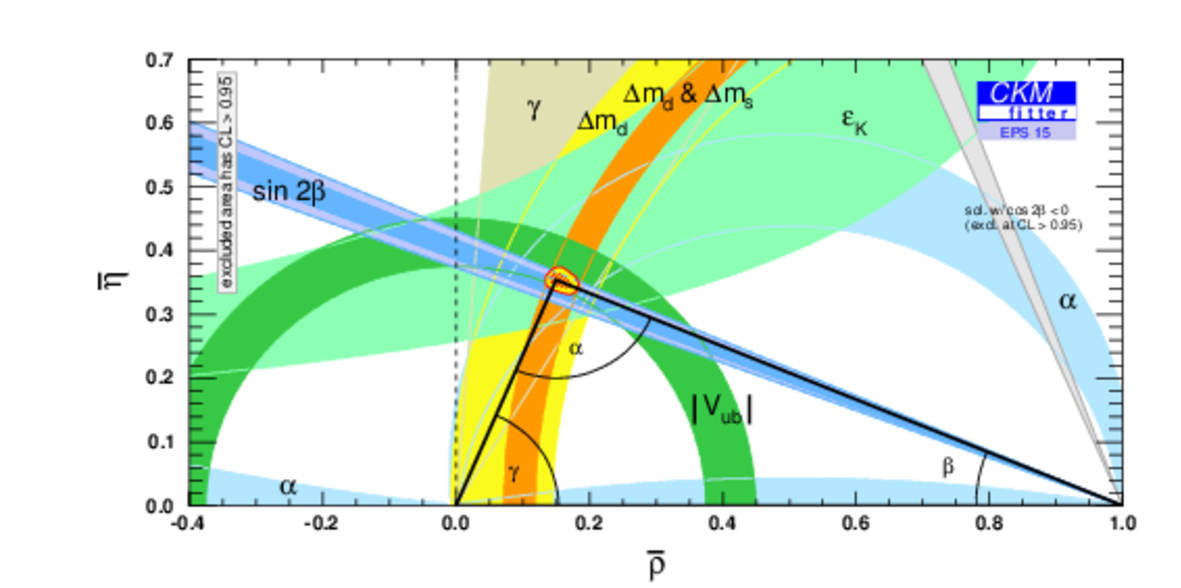
\includegraphics[width=8.5cm]{rhoeta_small_global.pdf}
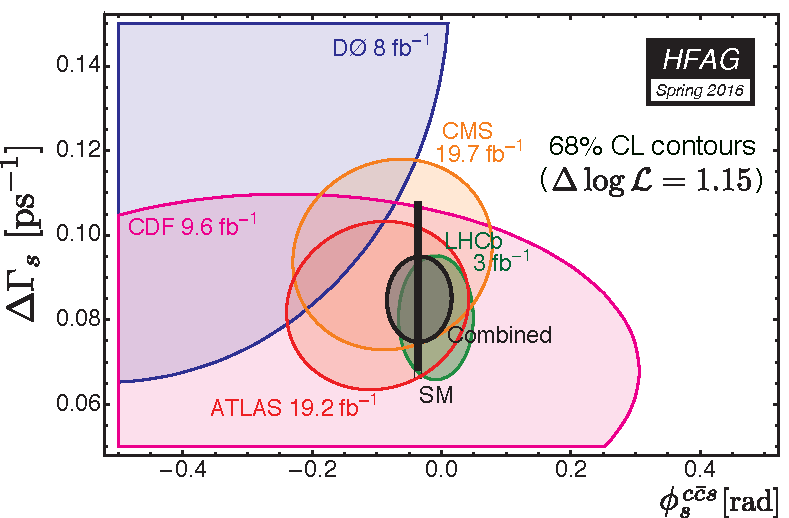
\includegraphics[width=7.cm]{hfag_Spring2016_DGsphis_zoom.pdf}
\end{center}
\caption{Left plot: the current status of the CKM unitarity triangle test from the CKMFitter collaboration~\cite{Charles:2004jd}.  Right plot: 68\% CL regions in $B^{0}_{s}$ width difference $\Delta\Gamma_{s}$
and weak phase $\phi_{s}$ obtained from individual and combined CDF, D0,
ATLAS, CMS and LHCb likelihoods of $B^{0}_{s}\to J/\psi\phi$, $B^{0}_{s}\to
J/\psi KK$, $B^{0}_{s}\to J\psi\pi\pi$ and $B^{0}_{s}\to D_{s}^{+}D_{s}^{-}%
$. The expectation within the SM is shown as the black rectangle. }%
\label{figphis}%
\end{figure}



%
%\section{Charmless $b$ Hadron Decays}
%\label{sec:charmless}
%
%The study of of $b$-hadron decays to hadronic final states with no charmed particles allow for a rich array of studies. A few examples are the measurements of branching fractions, $CP$ asymmetries, weak and strong phases and the CKM angles; they probe the dynamics of weak and strong interactions. The typical branching fractions of these modes are below $10^{-5}$ and thus their analyses are feasible only with large data samples and the use of powerful tools to reject background. The LHCb experiment is an adequate experimental environment for these analyses, offering the possibility to study decays of light $B$ mesons, $B_s$ mesons and $b$ baryons.
%
%In particular, $CP$-violation related studies of charmless $b$-hadron decays have a number of theoretical applications and that provide a probe to new physics, along the lines described in Sec.~\ref{sec:$CP$v}.
%For instance, the decays \BdtoKsPiPi and \BdtoKsKK are dominated by \btoqqbars ($q = u,d,s$)
%loop transitions.
%Mixing-induced \$CP$ asymmetries in such decays are predicted to be approximately
%equal to those in \btoccbars transitions, \eg $\Bd\to\jpsi\KS$, by the
%Cabibbo-Kobayashi-Maskawa mechanism~\cite{Cabibbo:1963yz,Kobayashi:1973fv}.
%However, the loop diagrams that dominate the charmless decays can have
%contributions from new particles in several extensions of the Standard Model,
%which could introduce additional weak phases~\cite{Buchalla:2005us,Grossman:1996ke,London:1997zk,Ciuchini:1997zp}.
%A time-dependent analysis of the three-body Dalitz plot allows measurements of
%the mixing-induced \$CP$-violating
%phase~\cite{Dalseno:2008wwa,Aubert:2009me,Nakahama:2010nj,Lees:2012kxa}. 
% The current experimental measurements of \btoqqbars decays~\cite{HFAG} show
%fair agreement with the results from \btoccbars decays (measuring the weak
%phase \Pbeta) for each of the scrutinised \$CP$ eigenstates.
%There is, however, a global trend towards lower values than the weak phase
%measured from \btoccbars decays.
%The interpretation of this deviation is made complicated by QCD
%corrections, which depend on the final state~\cite{Silvestrini:2007yf} and
%are difficult to handle.
%An analogous extraction of the mixing-induced \$CP$-violating phase in the
%\Bs system ($\beta_s$) will, with a sufficiently large dataset, also be possible with
%the \BstoKsKPi decay, which can be compared with that from, \eg
%$\Bs\to\jpsi\phi$.
%
%An impressive harvest of results from charmless hadronic $B$ mesons decays was obtained by the $B$ factories. Several french groups participated in these studies within the BaBar experiment, and in particular, a part of the present LPNHE-LHCb group. The LHCb experiment is already playing an important role in this area of physics, with the participation of the LPC and LPNHE groups. Both have contributed to the LHCb analysis of the decay modes \BstoKshhp ($\had^{(\prime)} = \pi, K$) with $1$~fb$^{-1}$ of data, which are being pursued with $3$~fb$^{-1}$.  In particular they are performing amplitude analyses (aka Dalitz-plot analyses) of \BdtoKsPiPi and \BdtoKsKK decays. At LHCb, the first step of the charmless $b$ hadron decays physics programme is to establish the signals of yet unobserved rare modes. The only yet-unobserved \BstoKshhp mode is \BstoKsKK. The LPC group also performs analyses of $B_s \to \rho^0 \rho^0$, and $\Lambda_b^0 (\Xi_b^0) \to p \had \had^{\prime}\had^{\prime\prime}$ decays.
%
%All the analyses mentioned above provide a long-term physics programs that can profit from the LHCb upgrade. These analyses proceed in increasingly complex steps, which become more and more sensitive to new physics observables with the growing dataset, and with more observed decay modes. One of the long-term goals is to perform full flavour- and time-dependent Dalitz-plot analyses of the \BstoKshhp modes to the measure the weak phases $\beta$ and $\beta_s$. Recent theoretical and experimental activity has focused on the determination of the CKM angle \Pgamma from charmless $B$ meson decays using and refining the methods proposed in Refs.~\cite{Ciuchini:2006kv,Gronau:2006qn,Bhattacharya:2013cla}. The LPNHE group is checking the applicability of the method described in the last reference to the LHCb physics analysis. Moreover, with the upgrade of LHCb, more modes, eventually with more neutral hadrons, are being considered.

%\documentclass[12pt,epsf,amssymb,qsymbols]{article}
%\usepackage{tabularx}
%\usepackage{array}
%\usepackage{graphics}
%\usepackage{graphicx}
%\usepackage{psfrag}
%\usepackage{epsfig}
%\usepackage{amsmath}
%\usepackage{amssymb}
%\usepackage{ulem}
%%\usepackage{figlatex}
%\usepackage{rotating}
%\usepackage{colortbl}
%\usepackage{tabularx}
%\usepackage{longtable}
%\usepackage{multirow}
%\makeatletter
%
%
%%%%%%%%%%%%%%%%%%%%%%%%%%%%%%% Textclass specific LaTeX commands.
%\usepackage{verbatim}
%%\usepackage{citesort}
%
%\setlongtables
%
%%%%%%%%%%%%%%%%%%%%%%%%%%%%%%% User specified LaTeX commands.
%%###################################################
%%###################################################
%%######## D E F I N I T I O N S ####################
%%###################################################
%%###################################################
%\setlength{\oddsidemargin}{0pt}
%\setlength{\textwidth}{16.2cm}
%\setlength{\topmargin}{-0.35in}
%\setlength{\textheight}{22.6cm}
%\newcommand{\msbar}{{\overline{\rm MS}}}
%\newcommand{\ri}{{\rm RI-MOM}}
%\newcommand{\csw}{c_{\mbox{\scriptsize \rm SW}}}
%\newcommand{\bea}{\begin{eqnarray}}
%\newcommand{\eea}{\end{eqnarray}}
%\newcommand{\beq}{\begin{equation}}
%\newcommand{\eeq}{\end{equation}}
%\newcommand{\ec}{\end{center}}
%\newcommand{\bc}{\begin{center}}
%\newcommand{\gev}{{\rm GeV}}
%\newcommand{\mev}{{\rm MeV}}
%\newcommand{\lr}{\leftrightarrow}
%\newcommand{\pdir}{p\kern -5.2pt\raise 0.2ex\hbox {/}}
%\newcommand{\one}{1\hspace*{-1.05mm} \hbox {I}}
%\newcommand{\vdir}{v\kern -5.75pt\raise 0.15ex\hbox {/}}
%\newcommand{\kdir}{k\kern -5.75pt\raise 0.15ex\hbox {/}}
%\newcommand{\epsdir}{\epsilon\kern -5.0pt\raise 0.15ex\hbox {/}}
%\newcommand{\bvdir}{\bar{v}\kern -5.75pt\raise 0.15ex\hbox {/}}
%\newcommand{\Ddir}{D\kern -7.75pt\raise 0.20ex\hbox {/}}
%\newcommand{\Adir}{A\kern -7.75pt\raise 0.20ex\hbox {/}}
%\newcommand{\ldir}{l\kern -5.0pt\raise 0.2ex\hbox{/}}
%\newcommand{\varepsdir}{\varepsilon\kern -5.5pt\raise 0.15ex\hbox{/}}
%\newcommand{\vare}{\varepsilon}
%\newcommand{\etc}{{\it etc}}
%\newcommand{\cs}{{\cal S}}
%\newcommand{\cb}{{\cal B}}
%\newcommand{\nf}{{N_{\rm f}}}
%\newcommand{\kkbar}{K^0-\bar K^0}
%\def\bpi{$B \rar \pi \ell \nu$}
%\def\bk{B_K}
%\newcommand{\m}[0]{\phantom{$-$}}
%\newcommand{\z}[0]{\phantom{0}}
%\newcommand{\n}[0]{\cellcolor[gray]{0.85}}
%\def\ds{\displaystyle}
%\def\negcdot{\negmedspace\cdot\negmedspace}
%\newcommand{\nn}{\nonumber}
%\makeatother
%
%\begin{document}
% 
%\setcounter{footnote}{0}
%%%%%%%%%%%  Section 1
\section{Rare, radiative and semileptonic $B$ decays}

The LHCb collaboration has produced a large set of results related to the exclusive $b \to s\ell \ell $ decay modes and their results are currently dominating the field. 
In the special case of the $\cb(B_s\to \mu\mu)$, the CMS collaboration is also significantly contributing and after combining the two results, 
it turned out that the long searched $\cb(B_s\to \mu\mu)$ is only slightly lower than, but compatible with, the value
predicted in the Standard Model (SM). The $\cb(B_d\to \mu\mu)$ decay has also been seen, its branching ratio is also compatible with the value predicted by the SM. 

\par
Joint work between experimentalists ans theorists have allowed to identify an ensemble of observables which are
at the same time sensitive to the couplings to different possible sources of New Physics (NP) and as immune as possibie to non factorizable QCD effects. 
In this framework, after comparing the experimental values of those observables, as well as of $\cb(B\to K \mu\mu)$ and $\cb(B_s\to \phi \mu\mu)$, with the theoretical estimates derived in the SM, 
one finds considerable discrepancies (of the order of 3 to 3.5 standard deviations). 
It appears, however, that the most significant discrepancies occur near the charm production threshold, a region notoriously difficult for theoretical 
description of these decays because it requires an accurate estimate of the hadronic matrix element of a non-local operator corresponding to disconnected $c\bar c$-diagrams which 
cannot be computed by means of numerical simulations of QCD on the lattice. For that reason, as of now, it is not clear whether the current discrepancies are due to the lack of theoretical 
control of the $c\bar c$ contributions, or they indicate the presence of NP couplings. If the second option is adopted, the angular observables of $B\to K^\ast \mu\mu$ and $B_s\to \phi \mu\mu$ 
decay modes provide very stringent constraints on the scenarios of physics BSM. It is important to note that these results were confirmed for the $B^0\to K^\ast \mu\mu$  analysis by the BELLE collaboration. 
On top of the very rich set of results involving muons, LHCb has also performed an angular analysis  of the $B^0\to K^\ast e e $ decay mode in the low dilepton invariant mass region. The results found there are in agreement with SM but currently quite limited in statistics.  

Another experimental result which has also provoked some interest in the flavor physics community is that $R_K = \cb(B\to K\mu\mu)/\cb(B\to Kee)_{{\rm low}-q^2}$ was found to be $2.6\sigma$ smaller than  predicted in the SM, which suggests the violation of universality of the coupling to leptons (LFUV). Such a puzzling phenomenon should be scrutinized with higher statistics and tested in other similar situations, 
such as $R_K$ at high-$q^2$'s, $R_{K^\ast , \Lambda^{(\ast )}}$ at both low- and high-$q^2$'s. This observation is adding to an already noted problem of $R_{D^{(\ast)}}=  \cb(B\to D^{\ast}\tau\nu_\tau)/\cb(B\to D^{\ast}\mu\nu_\mu)$ for which the experimental result, first measured at the $B$-factories and then confirmed at LHCb, is $(2\div 4)\sigma$ larger than predicted in the SM. There are very few phenomenologically viable theoretical scenarios of NP which can simultaneously explain that $R_K^{\rm exp}<R_K^{\rm SM}$ and that $R_{D^{(\ast )}}^{\rm exp} > R_{D^{(\ast )}}^{\rm SM}$. To further understand the origin of the LFUV one can envisage doing the angular analysis of all the mentioned decay modes, and from the ratios of angular observables check whether or not a similar size of the LFUV is indeed observed. 
Furthermore, to facilitate a comparison with theory it is more sound to compare $B_s\to D_s^{(\ast)}\ell \nu_\ell$ because the theoretical uncertainty related to the chiral extrapolation in the light valence quark on the lattice is completely avoided in this way. Moreover, the emission of soft photons can differently affect $B^- \to D^{0 (\ast)}\ell^- \bar \nu_\ell$ and $B^0 \to D^{- (\ast)}\ell^+ \nu_\ell$, the modes which are usually averaged. Such a problem is much less significant of one works with $B_s\to D_s^{(\ast)}\ell \nu_\ell$ decays. 

Most of the models pretending to describe the LFUV effects allow for the lepton flavor violation (LFV) too. For that reason it is of great interest to measure the LFV modes such as $B_s\to \mu \tau$, $B\to K^{(\ast )}\mu \tau$,  $B_s\to \phi \mu \tau$, which can now be probed thanks to the large statistics achievable at the LHC. Experimental bounds on $\cb(B_s\to \mu e)$ and $\cb(B_s\to K^{(\ast )} \mu e)$ can be greatly improved thanks to the unprecedented statistics of the LHC data. These results can be very useful for phenomenology of the LFV decays and for the bigger picture that could ultimately lead to a theory of flavor of quarks and leptons. 


The work of this part of GDR will be carried out within two working groups (theory and experiment) and the outcome of their works and discussions will be presented at the annual workshops that 
will unite both the theorists and experimenters and which will be organized following the agenda described below.
\begin{enumerate}
\item Year One: Workshop on the LFUV in $B$ and $B_s$ decays\\ 
During this workshop the theorists will discuss a general scenario of NP, in an effective field theory approach, and isolate the observables which are most sensitive 
to the couplings to the vector (scalar) and/or axial (pseudoscalar) operators. Experimenters and theorists will elaborate on the feasibility of the distribution of $B_{(s)}\to D_{(s)}^\ast  \ell \nu_\ell$ 
according to the polarization of the outgoing vector meson. Furthermore, a contact with other leptonic observables should be made in order to test several plausible scenarios of NP which 
result in LFUV.

\vskip .6cm 

\item Year Two: Workshop on the angular distribution of various decay modes\\ 
With the new and more accurate experimental data it becomes mandatory to assess the hadronic uncertainties on the theory side. Lattice QCD and the QCD sum rule practitioners will try and 
evaluate the size of theoretical errors and discuss the appropriate methodology on how to account for various sources of systematic uncertainties. 
An other interesting subject could be the angular analysis of $B^0\to K^\ast \tau\tau$ and the study of new observables taking into account the direct access to the $tau$ polarization.
The study of $b \to s \ell \ell$ transition in b-baryons  is quite new and the identification of interesting observables for the $\Lambda_b \to \Lambda^\ast \mu\mu$ may be interesting.  
Possible phenomenological ideas on how to relate the hadronic quantities in several decay modes will be discussed as they might be helpful in cancelling a large part of hadronic uncertainties.
Ideas on how to treat the non-resonant $c\bar c$-contributions would be very welcome. Participants will also address the question {\it ``Which physics BSM?"}

\vskip .6cm 

\item Year Three: Workshop on the lepton flavor violation in $b$-decays\\ 
Revisiting the LFUV problem: discuss the new constraints on  $R_{K^{(\ast )}, D^{(\ast )}, \Lambda^{(\ast )}}$ obtained in Belle~II, and attempt drawing more accurate conclusions concerning the 
new physics scenarios. Focus then on the LFV modes and on interpretation of the results found by LHCb. The issues related to the identification of $\tau$ in the final state should be revisited. 
Work on the package of codes that would include all possible constraints relevant to the LFV at low and high energy and see what are the lessons one can learn about the Yukawa sector from the data. 

\vskip .6cm 

\item Year Four: Workshop on the relation to Higgs \\ 
Assess the current situation concerning the extraction of the Yukawa couplings from experimental data. In what way those data can be related to the low-energy physics observables and 
$b$-decay observables in particular. In order to address the issue of ``{\it Which theory of flavor?}" we will try and combine the searches made at Belle~II with those made at NA62 and KOTO experiments. 
Address the issue of (in)compatibility of the conclusions found in the Yukawa sector through the low-energy experiments with the LHC findings at the TeV-scale. 

\end{enumerate}
%\end{document}



\section{Charm and kaon physics}

\label{sec:CharmAndKaon}
In the LHC collisions, a large part of the proton-proton cross section goes into charm and strange quarks production.  
The $c \bar{c}$ cross-section is roughly 10\% of the total inelastic cross-section, so that charm hadrons are produced extremely copiously. Their short but measurable decay times make them relatively simple to reconstruct and separate from background. The LHCb detector has developed dedicated triggers registering  large samples of charm hadron decays and is currently exploring the best strategy to collect a large quantity of kaon decays. In fact, charm and kaon physics provides complementary insights into flavour  physics to the ones obtained from the $b$ sector.  In the context of the GDR, we will profit of the previous experimental experience of the French community in these domains to try to extract the most of the physic potential for charm and kaon physics within LHCb, but we will of course follow the results of the currently ongoing dedicated experiments like NA62. Their is a clear interplay with the studies concerning $CP$ violation and rare decays in the charm and kaon sectors with those in the $b$ sector. Thanks to the GDR, the  community will  have the possibility to come together and analyze all the results of flavour  in a general framework. 

\subsection*{Charm physics}
 Theoretically, $CP$ violation in charm mesons is expected to be very small
because the GIM mechanism is much more powerful for $c\rightarrow u$
transitions than for $s\rightarrow d$ or $b\rightarrow s,d$ transitions. The $CP$ violation in decay is therefore expected to occur at below the per mil level in the SM.  
At the same time, NP need not to respect this peculiar feature, so these
observables provide almost-null tests of the SM.  
Additionally, compared to beauty or strange hadrons, the mixing of neutral charm hadrons is slow, with both the $x = \Delta m/\Gamma$ and $y = \Delta \Gamma/ (2\Gamma)$ parameters at around the percent level.

 The $CP$ violation in charm decays has not been observed so far, and the existing experimental limits are at the few per mil level. The theoretical predictions of charm $CP$ violation are difficult as long distance contributions dominate; $CP$ violation in decay close to the present experimental limits could be accommodated within the SM or could be signs of NP, and a progress on the theory side is required to disentangle the two. Similarly, in the case of mixing, or $CP$ violation in the interference of decay and mixing, more precise experimental results are needed to stimulate progress on the theoretical predictions. The current bounds are shown in figure~\ref{fig charm} on the left.

In addition, charmed hadrons are also an interesting place to study rare and forbidden transitions, for example flavour  changing neutral currents (FCNC) or lepton number violating decays. The most recent studies of charmed hadron decays within the French community were performed on the rare decays $D_{(s)}^+ \to \pi \mu\mu$~\cite{Aaij:2013sua} with same sign muons and $D^0 \to K \pi\mu\mu$~\cite{Aaij:2015hva}. The former is of interest because the copious production rate of charmed hadrons allows effective limits to be placed on Majorana neutrinos. The latter is the charmed counterpart of $B\to K^*\mu\mu$ and has now been observed for the first time by LHCb, albeit within a dimuon $q^2$ region dominated by the $\omega$ and $\rho$ resonances. It should in principle share much of the same phenomenology of $B\to K^*\mu\mu$,  with the complication of much higher backgrounds from decays to hadronic resonances (such as $\rho$) which subsequently decay to dimuon pairs. Once that a large signal yield becomes available, an angular analysis will be of prior interest. 

\subsubsection*{Plans for the GDR}
In the upcoming period, the most critical work  in the charm field will be the following.
\begin{itemize}
\item Improve the limits on $CP$ violation in charm, both in decay and the interference of mixing and decay, as well as  make ever more precise measurements of charm mixing parameters using both the $D\to hh$ and $D\to K_s hh$ decay modes with the full Run2  LHCb dataset. \item LHCb should obtain large samples of FCNC decays such as $D^0\to K \pi\mu\mu$.  Potentially this will allow for an observation of the non-resonant (in the dimuon spectrum) decay and a measurement of angular observables similar to the ones which characterise $B\to K^*\mu\mu$. 
\item Make more precise measurements of charm hadron lifetimes, in particular in the less well understood baryon sector. This could aid the development of heavy quark effective theory (HQE) tools and techniques required to eventually obtain precise SM predictions for mixing and $CP$ violation in the charm sector.
\end{itemize}



\subsection*{Kaon physics}

  Kaon physics is the birthplace of $CP$ violation, and has played a central
role in establishing the CKM picture in the past five decades. Kaon mixing and decays belong traditionally to the most constraining processes for physics beyond the SM. Currently, two main aspects are relevant for our proposed plans. First, advances in lattice QCD may well help to finally shed new light on the precisely measured direct $CP$ violation parameter $\epsilon^{\prime}_K$. Over the last years, lattice-QCD progress in the evaluation of $K \to \pi \pi$ matrix elements has been no less than astonishing. As a result, a mature, first-principle SM calculation of $\epsilon^\prime_K/\epsilon_K$ is no more just a dream. We should emphasize that this quantity, along with $\epsilon_K$ itself, is among the most formidable probes of physics beyond the SM, as it is able to probe NP scales as large as $10^{4}$ TeV. Second, theorists will be following closely the NA62 experiment, which aims at observing the ultra-rare and ultra-clean $K^{+}\rightarrow\pi ^{+}\nu\nu$ decay. The potential of this experiment, as well as of KOTO for the corresponding channel with a neutral pion, is shown in figure~\ref{fig charm} on the right.  Any hint of discrepancy with the SM in either of the $K$-physics quantities mentioned above would have implications for the other meson sectors.

In addition, the discrepancies found in recent LHCb and $B$-factory data, in particular in the quantity known as $R_K$ \cite{Aaij:2014ora}, provide motivations for searches of certain $K$ decays, in particular lepton-flavour violating  ones of the kind $K \to (\pi) e \mu$. In fact, $R_K$ may be naturally explained by a Fermi-like, TeV-scale new interaction involving third-generation quarks and leptons only \cite{Glashow:2014iga}. At the  energy scales of the decaying mesons, this interaction will produce, along with LFUV effects such as $R_K$, also LFV $B$ decays, whose natural magnitude can be estimated to be in the ballpark of $10^{-8}$ by just using the departure of $R_K$ from unity \cite{Glashow:2014iga}. That argument can be extended to $K$ decays as well, in particular those of the kind $K \to (\pi) \ell \ell'$ such as $K_L \to e^\pm \mu^\mp$ and $K^+ \to \pi^+ e^\pm \mu^\mp$. Limits on these modes are more than ten years old: $\mc B(K_L \to e^\pm \mu^\mp) < 4.7 \times 10^{-12}$ \cite{Ambrose:1998us}, $\mc B(K^+ \to \pi^+ e^- \mu^+) < 1.3 \times 10^{-11}$ \cite{Sher:2005sp}, $\mc B(K^+ \to \pi^+ e^+ \mu^-) < 5.2 \times 10^{-10}$ \cite{Appel:2000tc}. Theoretically, their expected magnitudes can be estimated after suitably normalizing them to cancel phase-space factors \cite{Cahn:1980kv}. The NP flavor structure can further be specified by using, for definiteness, flavor models proposed in connection with the $R_K$ result, e.g. \cite{Guadagnoli:2015nra,Boucenna:2015raa},   obtaining:
\be
\label{eq:KLemu}
\mc B(K_L \to e^\pm \mu^\mp) \approx 6 \times 10^{-14}~, \\
\mc B(K^+ \to \pi^+ e^\pm \mu^\mp) \approx 3 \times 10^{-15}~.
\ee
While the $K^+$ LFV mode is clearly too suppressed, the $K_L$ one has a branching ratio close to $10^{-13}$. Such a rate may actually well be reachable at the NA62 experiment. Concerning LHCb, it should be noted that, although $K$ mesons are produced copiously, their lifetimes are typically too long for the detector size, with the exception of the $K_S$. A dedicated study is thus necessary to understand the actual LHCb capabilities for the above decays.

\subsubsection*{Plans for the GDR}

The above considerations can be translated in a number of interesting directions to be pursued in the framework of the GDR.

\begin{itemize}

\item Closely follow the impressive progress in the lattice-QCD evaluation of direct and indirect CP violation in the kaon sector. The French community has a tradition in lattice QCD and in kaon physics, and can play a leading role in establishing possible discrepancies in the mentioned quantities, and in their interpretation.

\item The meetings organized in the context of the present GDR will allow to invite  members of the NA62 collaboration, giving the opportunity to have regular exchanges with them. In this way our network will  follow closely the progress in the search of the $K^+ \to \pi^+ \nu \bar \nu$ decay and of the LFV decays of $K$ mesons.

\item An open question is, as mentioned, the possible reach of LFV $K$ decays by LHCb itself. Optimistic remarks on this possibility actually emerged in informal discussions  preceding the writing of the present document. This possibility deserves a dedicated study, and the GDR will be instrumental to frame progress in this direction.

\end{itemize}



\begin{figure}[!htb]
\begin{center}
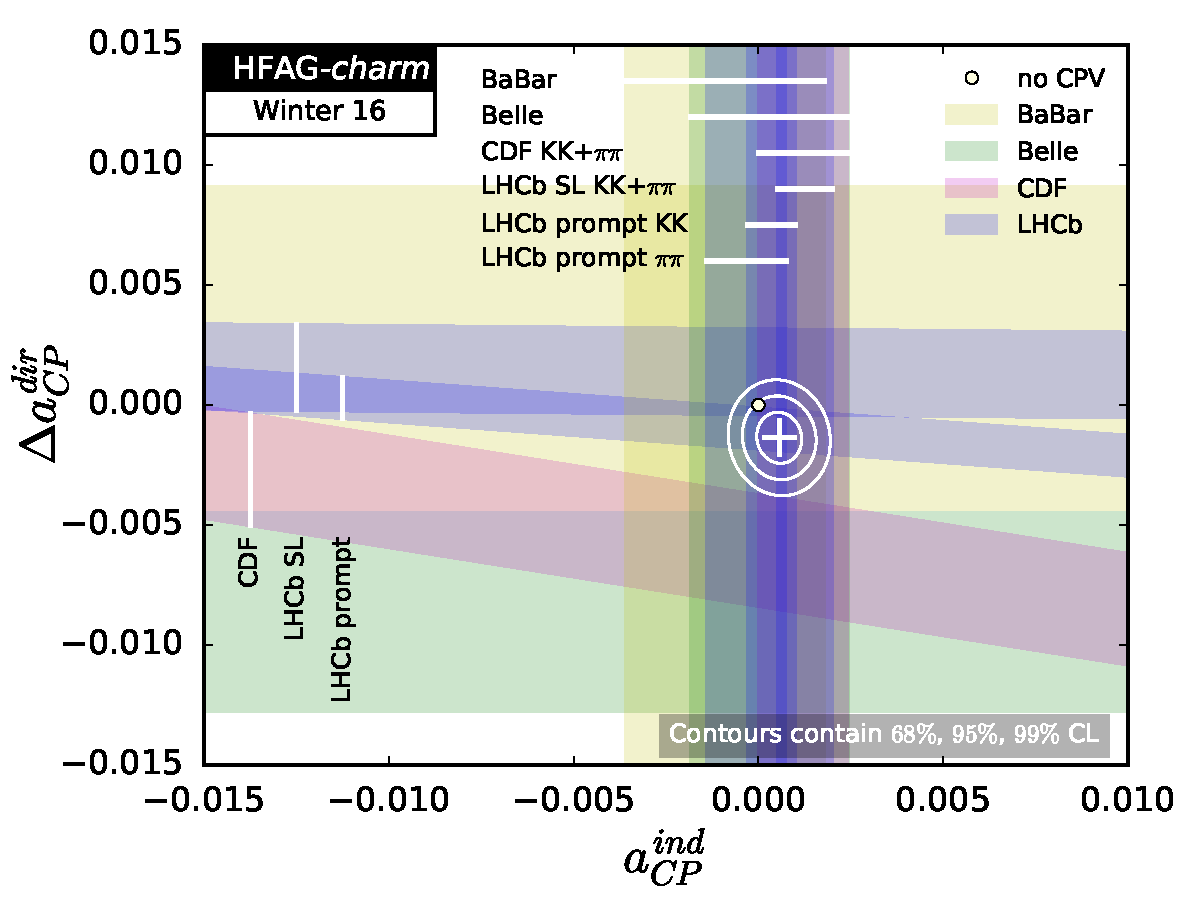
\includegraphics[width=7.5cm]{./deltaACP_AGamma_fit_Winter16.pdf}
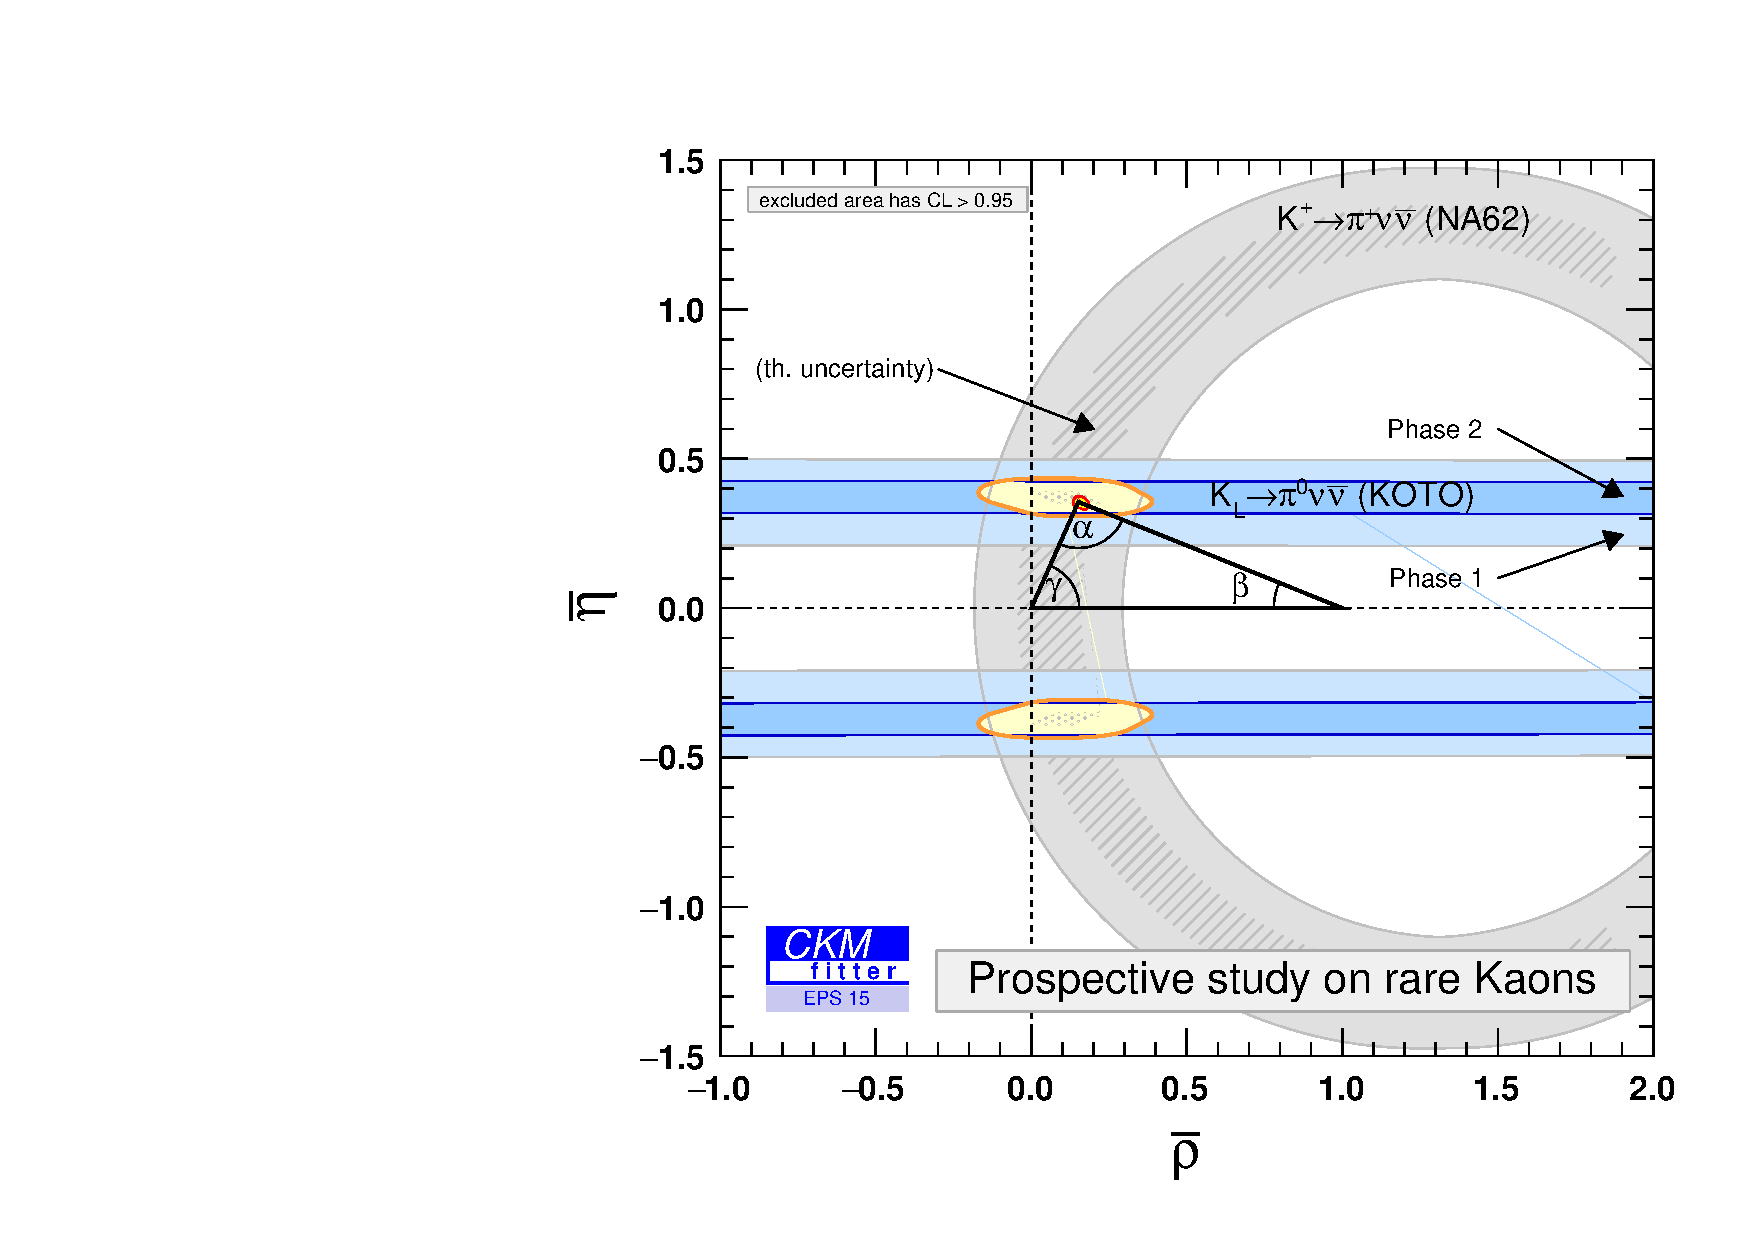
\includegraphics[width=7.5cm]{KbothPibothNuNu_RhoEta.pdf}
\end{center}
\caption{Left plot: summary of the current constraints on direct and indirect $CP$ asymmetry in the charm sector; the overall picture is, with the present uncertainties, consistent with no $CP$ violation observed in the $D$ mesons sector. Right plot: Constraints in the $(\bar{\rho}, \bar{\eta})$ plane, using a prospective scenario for the NA62 and KOTO experiments, from the CKMfitter group . For NA62, a measurement of $\mc B(K^{+}\rightarrow\pi ^{+}\nu\nu)$ with a 10\% accuracy is assumed; for its corresponding constraint (light gray), the theoretical contribution to the uncertainty is indicated by the dashed region. For KOTO, a two-step prospective scenario is assumed: first, a 3$\sigma$ evidence for the $\mc B(K^{+}\rightarrow\pi ^{0}\nu\nu)$ (Phase 1, lighter blue), followed by a later measurement of $\mc B(K^{+}\rightarrow\pi ^{0}\nu\nu)$  with 10\% accuracy (Phase 2, darker blue). For the combined NA62+KOTO constraint, the theoretical contribution to the uncertainty is indicated with the dashed region.}%
\label{fig charm}%
\end{figure}




%\bibliographystyle{JHEP}
%\bibliography{charm_and_K}

%\end{document}


\section{Heavy Flavor Production and Spectroscopy }

% We were thinking that it might be best if the separate sections have
% some uniformity in the way they are constructed, so as a rough
% guideline (proposed by Olivier) maybe you could ai for something like
% this:
%
%  - general introduction and motivation
%  - past and current work in the French community
%  - proposed work in the 4 coming years
%
% Note that the general introduction and motivation shouldn’t be too
% general as there will be an introductory section earlier in the
% document. Also try and be somewhat specific if possible as to the
% (recent) past and current work going on within the French community
% and why there is a need to continue and strengthen this effort.
%
% As for the length there is no length limit defined by the CNRS.
% We had mentioned a page but in words I think about 800-1000 words
% per section would be appropriate. This is of course a very rough
% guideline so you don’t need to keep to it too strictly.

%\subsection{Introduction and motivation}

Quantum Chromodynamics (and the quark model out of which it grew)
is one of the fundamental building blocks of the Standard Model.
It has been extensively validated over the decades, and is
very well understood. However, due to the non-perturbative behaviour
that follows from the large self-coupling of low-energy gluons,
the practical implications of QCD are still
very much an active subject of research. This was vividly illustrated
in the realm of spectroscopy recently, when the first compelling
observation of pentaquark ($qqqq\bar{q}$) states was made by LHCb~[\cite{Aaij:2015tga}]
just over fifty years after their existence was predicted [\cite{GellMann:1964nj}].
This discovery came as a surprise to experimentalists and theorists alike:
the possible existence of such states was known, but the quark composition of
quasi-stable pentaquark resonances (let alone their masses, widths, and
production mechanisms) was not.

More broadly, results from QCD and strong physics are frequently
needed as inputs to other measurements or to their interpretation.
For example, there is considerable interest in the decays
$\Bbar \to D^{(*)} \lepton^- \neulb$: the ratio of branching fractions
(in a restricted region of phase space) for $\lepton=\muon$ and $\lepton=\tauon$
can be used to test lepton universality. The current world average,
combining results from LHCb, BABAR and Belle, is in tension
at the $4\sigma$ level with Standard Model expectations~\cite{bib:hfag}.
One of the important systematic uncertainties in this measurement
is associated with the spectrum and properties of excited charm resonances $D^{**}$,
which could contaminate the final state with feed-down from
$\Bbar \to D^{**} \lepton^- \neulb$: here, input from spectroscopy is
needed for the measurement itself. There are numerous instances
in which QCD input is needed for the interpretation of measurements,
notably for $\Bz \to \Kstarz \mup \mun$ in which local tensions of
$3\sigma$ were seen by LHCb in two regions of phase space~[\cite{Aaij:2015oid}],
corresponding to an overall tension of $3.4\sigma$ with the SM
prediction of~\cite{Descotes-Genon:2014uoa}. The significance of the
tension depends strongly upon the SM theory prediction and its
uncertainties. To take a third and final example, QCD processes are
an inherent background to all physics at the LHC, and in some cases
Monte Carlo predictions of their spectrum need to be included in the
fit itself. Tuning of the Monte Carlo models requires not only work
from the phenomenology community but also measurements of production
cross-sections across a range of transverse momentum and
pseudorapidity.

%\subsection{(Past and current work in the French community)}

% Alphabetic ordering: CPPM > LPC > LAL > LAPP > LPNHE

The HEP community in France is engaged in this field, both on
the experimental and theory sides. For practical reasons most
experimental measurements have come from LHCb in recent years.
LHCb-France has been involved on multiple fronts:
spectroscopy of exotica (LAL, LAPP, LPNHE),
spectroscopy of non-exotic resonances (LAL, LPNHE),
and measurements of production rates (CPPM, LAL, LAPP, LPNHE).
This list is not exhaustive, and there are far too many
results to discuss them individually; purely by way of
illustration we point to recent contributions by French groups to
%
studies of exotic 4- and 5-quark resonances
[\cite{Aaij:2016ymb}, \cite{Aaij:2014jqa}],
%
discoveries of two $\Xi_b$ resonances and precise measurements
of their mass splittings [\cite{Aaij:2016jnn}, \cite{Aaij:2014yka}],
%
and measurements of the $J/\psi$ production cross-section
with the new 13\,TeV LHC data
[\cite{Aaij:2015rla}].
Numerous theory groups are also actively involved, and
we do not dare attempt an exhaustive list\footnote{
  In the author list of one review paper of heavy flavour
  production alone [\cite{Andronic:2015wma}],
  we counted eight French laboratories:
  IPNO, IRFU, LAL, LAPTh, LLR, LPC, LPSC, and SUBATECH.
}.
As well as hadron production, there is substantial French
expertise in spectroscopy theory. For example, the opening
theory review talk at the 
2014 Workshop on Heavy Quark Baryons at LHCb\footnote{
  \url{https://indico.cern.ch/event/317758/}
}, a workshop organised by LHCb to which external experts were invited,
was given by a member of IPNL. This is both recognition of
this expertise and an illustration of the demand for
productive theory-experiment crosstalk.

% Note that IPNL = IPN Lyon (vs IPN at Orsay)
%
% IPNL includes Jean-Marc Richard, an expert on hadron spectroscopy

% Note especially : arXiv:1407.8526

%\subsection{(proposed work in the 4 coming years)}

During the coming years, several analyses in this area are
planned by LHCb-France. These include studies in
beauty baryon spectroscopy following on from the observations
of three $\Xi_b$ resonances, searches for the doubly heavy
$\Xi_{cc}$ baryons, and measurements of production cross-sections
at new centre-of-mass energies (including the 13\,TeV Run-2
data and in heavy-ion collisions). Assuming that the $\Xi_{cc}$
searches are successful, they in particular will lead to fruitful
exchanges with theory: their masses and properties will have
immediate implications for QCD models, and theory input will be
very useful for the next step, namely observing and studying their
excitations.

% fin

\section{Interplay of quark and lepton flavour}

As previously highlighted, many of the observables whose experimental
measurements reveal lingering tensions with respect to the SM
theoretical expectations consist of a large variety of 
(very) rare processes, among them semi-leptonic
or leptonic meson decays.

Particularly interesting examples of
these are the semi-leptonic and leptonic $R_K$ ratios, 
$R_K = \cb(B\to K\mu\mu)/\cb(B\to Kee)_{{\rm low}-q^2}$ (exhibiting a 
$2.6\sigma$ deviation from its SM prediction), and 
$R_K^{\rm leptonic} = \cb(K\to \mu\mu)/\cb(K\to ee)$.
Both the latter observables could signal the violation of lepton flavour
universality, which might possibly be a consequence of charged lepton
flavour violation\footnote{For recent studies on $R_K^{\rm leptonic}$, see for
  example~\cite{Fonseca:2012kr,Abada:2012mc,Abada:2013aba}.}.   
 
Understanding these tensions (if confirmed) calls for extensions of the SM, 
leading to modifications of its flavour paradigm. While many New Physics
constructions address the hadronic sector, others aim at explaining 
the experimental tensions
from the leptonic point view. 
By itself, flavour violation in the charged lepton sector is an 
unambiguous signal of New Physics. The experimental effort
devoted to search for cLFV in a variety of processes 
(MEG, Mu2e, Mu3e, COMET, LHCb, SuperB, future FCC-ee and LC, ...)
implies that in the near future the 
different bounds will become much stronger, further lending hope to a
possible observation. 

From a theoretical point of view, it is also important to stress that
certain well-motivated constructions called upon to address the quark flavour
puzzle have unavoidable implications regarding lepton flavours as
well. 
Examples of such constructions include extended Higgs sectors
(several realisations of 2HDM, type II seesaw, ...),
extended gauge sectors 
(e.g., additional $Z^\prime$ bosons) or additional symmetries - flavour
symmetries, or gauge ones, such as left-right symmetric models -, and finally 
larger frameworks as general Supersymmetry, extra dimensional models and
Grand Unified Theories. 

In all cases, it is clear that one must 
carefully evaluate the possible contributions to the
distinct charged lepton flavour observables: these include 
purely leptonic processes, such as 
radiative $\ell_i \to \ell_j \gamma$, 3-body $\ell_i \to 3\ell_j$,
etc., or processes involving hadron as is the case of semileptonic 
tau decays (such as $\tau \to \ell_i$+light hadrons), leptonic and 
semileptonic $B$, $D$
and $K$ meson decays, ..., and finally Higgs and $Z$ flavour violating
decays.
The expected contributions must be 
confronted with the available (and soon to
be improved) bounds, which will further allow one to constrain the
parameter space of different theoretical models, possibly
impacting on the associated predictions regarding flavour
violation in the hadron sector. 
The synergy between the observables might allow to 
readily exclude some of these well-motivated scenarios, and 
possibly to discriminate among distinct realisations of 
flavour violating models 
(see, e.g.,~\cite{Abada:2014cca,Abada:2015zea,Abada:2015oba}). 

\medskip
It is important to stress that the
studies referred to above 
will clearly also have an impact on other flavour conserving 
observables, as is the case for the muon anomalous magnetic moment
$(g-2)_\mu$ 
or electric dipole moments of leptons. The exploration of these observables
(already foreseen in the present Scientific Proposal) might offer 
additional insight into the lepton and quark flavour puzzle.


\medskip
Considering the interplay between quark and lepton flavour
violation, combining the informations and data arising from each
sector, is thus relevant (and even mandatory!) to fully understand 
the underlying theory of flavour, and constrain - or even identify -
the New Physics model at its origin. 


%% %%%%%%%%%%%%%%%%%%%%%%

%% \bibitem{Fonseca:2012kr}
%%   R.~M.~Fonseca, J.~C.~Romao and A.~M.~Teixeira,
%%   %``Revisiting the $\Gamma(K \to e \nu)/\Gamma(K \to \mu \nu)$ Ratio in Supersymmetric Unified Models,''
%%   Eur.\ Phys.\ J.\ C {\bf 72} (2012) 2228
%% %  doi:10.1140/epjc/s10052-012-2228-2
%%   [arXiv:1205.1411 [hep-ph]].

%% \bibitem{Abada:2012mc}
%%   A.~Abada, D.~Das, A.~M.~Teixeira, A.~Vicente and C.~Weiland,
%%   %``Tree-level lepton universality violation in the presence of sterile neutrinos: impact for $R_K$ and $R_\pi$,''
%%   JHEP {\bf 1302} (2013) 048
%% %  doi:10.1007/JHEP02(2013)048
%%   [arXiv:1211.3052 [hep-ph]].

%% \bibitem{Abada:2013aba}
%%   A.~Abada, A.~M.~Teixeira, A.~Vicente and C.~Weiland,
%%   %``Sterile neutrinos in leptonic and semileptonic decays,''
%%   JHEP {\bf 1402} (2014) 091
%% %  doi:10.1007/JHEP02(2014)091
%%   [arXiv:1311.2830 [hep-ph]].

%% \bibitem{Abada:2014cca}
%%   A.~Abada, V.~De Romeri, S.~Monteil, J.~Orloff and A.~M.~Teixeira,
%%   %``Indirect searches for sterile neutrinos at a high-luminosity Z-factory,''
%%   JHEP {\bf 1504} (2015) 051
%% %  doi:10.1007/JHEP04(2015)051
%%   [arXiv:1412.6322 [hep-ph]].

%% \bibitem{Abada:2015zea}
%%   A.~Abada, D.~Becirevic, M.~Lucente and O.~Sumensari,
%%   %``Lepton flavor violating decays of vector quarkonia and of the $Z$ boson,''
%%   Phys.\ Rev.\ D {\bf 91} (2015) no.11,  113013
%% %  doi:10.1103/PhysRevD.91.113013
%%   [arXiv:1503.04159 [hep-ph]].

%% \bibitem{Abada:2015oba}
%%   A.~Abada, V.~De Romeri and A.~M.~Teixeira,
%%   %``Impact of sterile neutrinos on nuclear-assisted cLFV processes,''
%%   JHEP {\bf 1602} (2016) 083
%% %  doi:10.1007/JHEP02(2016)083
%%   [arXiv:1510.06657 [hep-ph]].



\section{Future experiments}

There are a large variety of future experiments at the intensity frontier starting or planning in the coming years. Here we have divided them into two categories:  flavour physics experiments which can indirectly probe high energy scales through precision measurements and experiments searching directly for physics beyond the SM. One of the role of the GDR will be to promote the discussions on  which are the priorities and the complementarities among the different physics topics, and which are the most promising experiments  where the French community should  contribute. The mix of data analysis and preparation of new experiments which will characterize the coming years,  illustrated indicatively by figure~\ref{timeline} for some of the experiments discussed in this proposal, will be a unique opportunity to ensure the continuity of the successful French involvement in the intensity frontier field.  


\subsection*{Future experimental programs related to $CP$ violation, rare decays of heavy flavours and lepton flavour violating processes}   

As far as $CP$ violation and rare $b$-flavoured hadrons or $\tau$ decays are concerned, the two main players at the horizon of 2025 are the  upgraded LHCb experiment at CERN and the Belle II experiment at KEK.  The synergy and complementarity between the two projects has been assessed clearly in the past and we should ensure within the GDR to follow the progress in both the collaborations. The involvement of France in LHCb is clearly established.  For Belle II, we can profit of the connexions among some members of the GDR with the KEK colleagues in the framework of the TYL/FJPPL (Franco-Japan Particle Physics Laboratory) and also of the current participation into the Belle II-Theory Interface Platform" (B2TIP: https://confluence.desy.de/display/BI/B2TiP+WebHome), a joint theory-experiment effort to study the potential impact of the Belle II program.

Several large or medium scale projects related to flavour physics are envisaged to probe physics beyond the SM. Among them, there are prospective studies to educate the possibility to run the LHCb spectrometer in the high luminosity phase of the LHC, or to make use of high intensity beam lines ({\it e.g.} SPS and FCC injectors)  with fixed target experiments, or  proposals for a Gamma Factory at CERN with a wide physics potential in the intensity frontier~\cite{Krasny:2015ffb}.

A possible long-term strategy for high-energy physics at colliders, after the exploitation of the LHC and its high luminosity upgrade, considers a tunnel of about 100 km circumference, which takes advantage of the present CERN accelerator complex. The Future Circular Collider (FCC) concept follows on the successful experience and outcomes of the LEP-LHC  experiments. A possible first step of the project is to fit in the tunnel a high-luminosity $e^+e^-$ collider aimed at studying comprehensively the electroweak scale with centre-of-mass energies ranging from the $Z$ pole up to beyond the $t \bar t$ production threshold. A  100 TeV proton-proton collider is considered as the ultimate goal of the project.  
FCC study groups have been formed in a design study hosted by CERN, aiming at a conceptual design report and a review cost in time for next European strategy milestone (2018-2019). The unprecedented statistics at the $Z$ pole, with ${\cal O}(10^{12-13})$ $Z$ decays potentially delivered by the high-luminosity $e^+e^-$ collider, can be studied in particular to explore further the flavour physics case at large.  

In that framework, several French teams, gathering small groups of experimentalists and phenomenologists, are contributing to the design study in flavour studies.  
There is a physics potential of the measurements of rare decays of $b$-hadrons, which can complement  the anticipated results from the current and foreseen $b$-physics programs (LHCb upgrade and SuperKEKB $B$-factory). In that respect, French contributions are mainly focused on rare electroweak penguins which are likely unique to the FCC: $B^0 \to K^*(892) \tau^+\tau^-$ and $B_s \to \tau^+ \tau^-$.   
The large statistics at the $Z$ pole can be used as well to scrutinize in particular Lepton Flavour Violating (LFV) $Z$ decays, which would serve as an indisputable evidence for NP, if seen. Heavy right-handed neutrals are natural candidates to explain LFV phenomena. They can be as well searched for directly at FCC-$ee$. A number of low energy experiment are addressing this very question through the search for LFV by muon capture on nuclei ({\it e.g.} COMET in Japan and Mu2e at FNAL) or the radiative decay of large ensemble of muons ({\it e.g.} MEG and Mu3e at PSI). 



\subsection*{Weakly interacting new light particles searches}

Weakly interacting new light particles, commonly called WISPs, have as two canonical candidates  hidden photons and axion-like particles. Experiments to search for these are in many cases very cheap, and can often recycle older experiments.  

The best motivated WISP is the QCD axion itself, which is expected to solve the strong $CP$ problem but is associated with new physics above $10^9$ GeV. Its mass may lie anywhere in the sub-eV range, and it is a very well-motivated dark matter candidate.   Axion-like particles (ALPs) are (pseudo)-scalars, perhaps cousins of the QCD axion but which do not obtain their masses from QCD. They are characterised by their coupling to photons in a Lagrangian term $\mathcal{L} \supset - \frac{1}{4} g_{a\gamma \gamma} a F_{\mu \nu} \tilde{F}^{\mu \nu}.$ ALPs are highly motivated from top-down constructions as generically arising when symmetries are broken at high scales, and also make attractive dark matter candidates. On the other hand, and perhaps most importantly, there have recently been several studies indicating possible discoveries of such particles in various astronomical observations: either as an explanation for excessive white dwarf cooling or anomalous transparency of the universe to gamma rays, and most excitingly as an explanation for the soft excess of X-rays from the coma cluster (at $200$ eV) and/or the oscillatory modulation of X-rays from the Perseus cluster (and even, perhaps, an explanation for an observed $3.55$ keV X-ray line). These hints all point to a very light ALP ($< 10^{-12}$ eV) with a coupling $g_{a\gamma \gamma} \sim \mathcal{O}(10^{-11} \div 10^{-12}) \mathrm{GeV}^{-1}.$ However, while this is a very interesting region to probe, such a particle could have a wide range of masses and couplings. 

Hidden photons are new (massive) gauge bosons which mix kinetically with the visible photon via a dimensionless kinetic-mixing parameter $\chi$. While one motivation of these is as a possible explanation for the $3\sigma$ discrepancy between the measured and calculated value of the muon dipole moment (requiring a hidden photon in the $\mathcal{O}(100)$ MeV range with $\chi \sim \mathcal{O}(10^{-3})$), they also appear generically in top-down constructions of physics beyond the SM. They have been proposed as perhaps the most natural force carriers for light dark matter particles, or could even make up the dark matter themselves. Recently, they have also been advocated to explain the 7$\sigma$ anomaly in the Be nuclear transition~\cite{Krasznahorkay:2015iga}.  

Intensity frontier experiments searching for WISPs either search for the particles as dark matter or attempt to directly produce them. In the dark matter case, the assumption that there is a large abundance of particles all around us greatly enhances the reach potential; on the other hand, for the very light ALPs this is unlikely to be the case. The dark matter searches consist of resonant cavities, helioscopes, and now many more exotic suggestions. Direct searches are broadly photon regeneration experiments (light shining through a wall), electron colliders or beam dumps. Flavour experiments like BaBar, Belle, KLOE and NA48 have been searching for and putting limits on hidden photons, and the flavour experiments effort will continue in the future also within LHCb and Belle II. Other upcoming dedicated experiments include:
%
\begin{itemize}
\item Axion haloscopes (magnetic resonant cavity experiments) ADMX-HF, YMCE and WISPDMX at the University of Washington, Yale and Hamburg respectively are all expected to report results soon, probing axion masses in the $\mu$eV range. 
\item The FUNK experiment in Karlsruhe uses a dish antenna to search for dark matter hidden photons;
\item The helioscope SHIPS at Hamburg searches for hidden photons produced in the sun;
\item The REAPR and ALPS-II photon regeneration experiments at Fermilab and DESY respectively will attempt to directly produce ALPs or hidden photons in the lab;
\item The IAXO helioscope at CERN, using a magnetic field to search for ALPs produced in the sun, is expected to operate over the next decade and there are significant synergies with the French community;
\item The SHIP  beam dump experiment using the SPS proton beam at CERN has a substantial input from French theorists and experimentalists.  It has the potential to search for messengers of NP portals and additional particles in the MeV-GeV range. Heavy neutral leptons (neutrino portal), dark photons (vector portal), light scalars (scalar portal) and pseudoscalars (ALP) can be searched for, as well as possible supersymmetric partners (neutralinos, sgoldstinos, axinos, saxions).  The SHiP beamline will be a perfect arena to plan experiments to detect the interactions of the above mentioned particles with matter, i.e. for an accelerator based direct dark matter search.
\item There will be electron beam-dump experiments HPS, DarkLight and MESA at SLAC, JLab and Mainz respectively, with the latter running in about 2020. These will provide high intensity competition to hidden-photon searches in the $10$-$1000$ MeV range.
\item The BMV experiment at Toulouse received ANR funding in 2014 to build phase two and complement its 2007 results. It can perform photon regeneration searches; it also included an X-ray regeneration experiment.
\item There is also a proposal to use the Tore Supra tokamak at Cadarache to search for ALPs. This would be particularly interesting to interact with the plasma physics community. 
\end{itemize}


\subsection*{Plans for the GDR}
One objective of the GDR will be to address the complementarity of the high intensity machines,  at large scale apparatus or low-energy experiments.  Discussions inside the GDR will help to identify the emerging technologies and those already mastered at IN2P3 which could play an important role for future experiments, helping the French groups to propose key contributions.  
Although it will not be possible to participate actively to all the experiments related to the field, it will be crucial within the GDR to discuss them and follow their advancement both from the theoretical and the experimental point of view. This will   eventually allow to select those more interesting for they scientific potential and in which a larger involvement will be beneficial for the French community at the intensity frontier. 



\begin{figure}[!htb]
\begin{center}
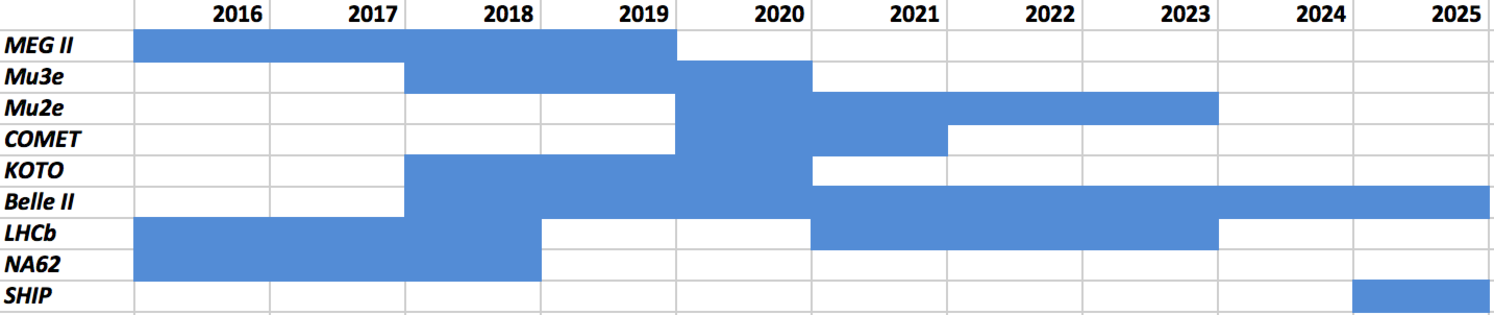
\includegraphics[width=12cm]{timeline.pdf}
\end{center}
\caption{Timeline of the data taking periods for some of the experiments discussed in the proposal. Although not comprehensive of all the activity ongoing in the intensity frontier field, and providing only  approximative dates, this timeline highlights the mixture of data taking and experiment preparation that will characterize the next years and that is one of the motivations of this GDR. }%
\label{timeline}%
\end{figure}




\section{Conclusion}
%The intensity frontier is a strategic approach to search for new physics.  Its validity is recognized at an international level and  it is a domain in which the French particle physics community is traditionally very active. Interesting and puzzling results are being produced by the experiments currently taking data, and further more are expected to come from the new generation of experiments that are starting or being planned. Theoretical progress are ensuring the precision of the currently performed tests, and additional clean observables are under investigation. 

%The French community working in this field recognizes the need of coming together to pursue these searches together with a renewed enthusiasm  and with a stronger collaboration between the experimental and the theoretical laboratories in France.   
%The GDR intensity frontier will be the place where we will be able to put together our experience, share our knowledge, renforce bounds and inspire new collaborations, ensuring that the French community continues to be competitive and focused on the most appealing topics of the field. It will additionally provide a forum to discuss the future of the field, and naturally promote the emergence of a young and dynamic generation of physicists. All this will allow to keep the current involvement and acquire an even higher visibility at a national and international level.

\textcolor{red}{The intensity frontier is a strategic approach to search for new physics: historically, many of the discoveries in high-energy physics came first as indirect evidence in high-intensity experiments, and only afterwards were confirmed by direct, targeted searches. The intensity frontier is, furthermore, a domain in which the French particle physics community has been traditionally very competitive.}

\textcolor{red}{In addition, and interestingly enough, tantalizing hints of beyond-SM effects exist in data from recent and present experiments at the intensity frontier, among the others LHCb, the B-factories, and experiments having measured the anomalous magnetic moment of the muon. More data on all of these discrepancies are expected to come from the new generation of experiments that are starting or being planned.}

\textcolor{red}{Theoretical progress will ensure the theory predictions to error-match the experimental accuracy of the planned experiments. Furthermore, additional clean observables have been proposed, and more are under investigation for the LHCb upgrade, for the Belle upgrade, for other flavor experiments outside B-physics, for example NA62, and for experiments aimed at new light-particle searches.}

\textcolor{red}{In short, we are in the favorable circumstance of interesting data flowing from experiments, more data expected to come, and of a French community with more than the critical size and the international reputation to be competitive in these searches and their interpretation. We therefore consider timely and strategic to form a "GDR Intensity Frontier". This  will allow for a financially well-defined structure to pursue collaborations within the community, beneficial among the other things to strengthen the interaction between the experimental and theoretical parties involved. Furthermore, the "GDR Intensity Frontier" will be the place to share our experience and our knowledge, reinforce existing bounds and inspire new collaborations, thereby ensuring that the French community stays competitive, and continues to focus on the most promising topics of the field. Finally, it will provide a forum to discuss the future of the field, and naturally promote the emergence of a young and dynamic generation of physicists active in the field, and educated in France. This latter point will be crucial to transmit the heritage of our community and to consolidate its international competitiveness over time.}



%----------------------------------------------------------------------------------------
%	BIBLIOGRAPHY
%----------------------------------------------------------------------------------------

\bibliographystyle{apalike}

\bibliography{sample}

%----------------------------------------------------------------------------------------


\end{document}